

\definecolor{listinggray}{gray}{0.9}
\definecolor{lbcolor}{rgb}{0.9,0.9,0.9}
\lstset{
	backgroundcolor=\color{lbcolor},
	tabsize=4,
	rulecolor=,
	language=matlab,
        basicstyle=\sffamily\footnotesize, %\scriptsize,
        upquote=true,
        aboveskip={1.5\baselineskip},
        columns=fixed,
        showstringspaces=false,
        extendedchars=true,
        breaklines=true,
        prebreak = \raisebox{0ex}[0ex][0ex]{
          \ensuremath{\hookleftarrow}},
        frame=single,
        showtabs=false,
        showspaces=false,
        showstringspaces=false,
        identifierstyle=\sffamily,
        keywordstyle=\color[rgb]{0,0,1},
        commentstyle=\color[rgb]{0.133,0.545,0.133},
        stringstyle=\color[rgb]{0.627,0.126,0.1},
}
\newcommand{\avg}[1]{\langle #1 \rangle}

\chapter{Implementation of a robust structured illumination
  reconstruction technique}
\label{sec:app_hilo}
\begin{summary}
  We implement a robust technique to computationally recover optically
  sectioned images from only two structured illumination images.
\end{summary}
\section{Simulated image acquisition}
As a test object we create a thick sphere shell, a line and a
rectangle. The sphere shell will provide out-of-focus light, which we
then try to remove. We simulate the illumination through an objective
with $\textrm{NA}=n\sin(\alpha)=1.4$ and oil ($n=1.518$) immersion
using coherent \unit[473]{nm} excitation light and incoherent
detection at \unit[520]{nm}.

The following listing shows how the image of the grating for
structured excitation is calculated. The $xz-$section of the result is
shown in \figref{fig:grating}. Due to coherent illumintation the
grating structure is repeated over nearly $\unit[6]{\mu m}$ in $z$
(Talbot effect).
\begin{lstlisting}
n=128;
nmperpixel=100; % one pixel is corresponds to 100nm
sz=2;
NA=1.4;
znmperpixel=sz*nmperpixel;
%% vector amplitude point spread function for excitation
asf=squeeze(kSimPSF({'lambdaEx',473;'na',NA;'ri',1.518;...
    'sX',n;'sY',n;'sZ',sz*n;...
    'scaleX',nmperpixel;'scaleY',nmperpixel;'scaleZ',znmperpixel;...
    'computeASF',1}));
P=6; % grating period
grat2d=(mod(xx(n,n),P)>(floor(P/2)-1))*1000;
grat=newim(n,n,sz*n); % copy the 2D grating into middle of volume
grat(:,:,(sz*n)/2)=grat2d(:,:);
kgrat=ft(grat);
imgratx=ift(kgrat.*ft(squeeze(asf(:,:,:,0)))); % field components
imgraty=ift(kgrat.*ft(squeeze(asf(:,:,:,1)))); % in sample for
imgratz=ift(kgrat.*ft(squeeze(asf(:,:,:,2)))); % coherent image
% intensity distribution in sample space:
imgrat=abs(imgratx).^2+abs(imgraty).^2+abs(imgratz).^2
\end{lstlisting}
\begin{figure}[htb]
  \centering
  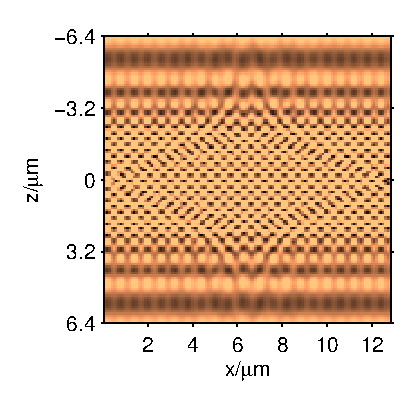
\includegraphics{../app_hilo/grating_xz}
  \caption{$xz-$cross section of the intensity distribution {\tt
      imgrat(:,64,:)} of the coherent image of the grating in sample
    space.}
  \label{fig:grating}
\end{figure}
The following listing shows how the sample object, i.e.\ the
fluorophore concentration, is generated.  The spherical shell is
calculated as the product of two Sinc functions in k-space and a
product with $r$ in real space. There is also a vertical line and a
rectangle. A slice through the simulated fluorophore concentration is
shown \figref{fig:input}~a). Note that the sphere is very faint but
it is the only of the three objects that is extended in $z$.

A shift by {\sf dz} in $z-$direction is done by multiplication with
$\exp(-ik{\sf dz})$ in k-space. This is only a good method to defocus
small distances {\sf dz} as the object will wrap around the borders.

\begin{lstlisting}
%% hollow sphere
kobj=sinc(rr(kpsf)./2).*sinc(rr(kpsf)./0.7); % in k-space
obj=rr(psf).*abs(ift(kobj)); % this is the sphere
maximum=max(obj);
obj(83:114,23:43,(sz*n)/2)=4*maximum; % rectangle in-focus rig ht top
obj(21:21,40:90,(sz*n)/2)=12*maximum; % in-focus line on the left
kobj=ft(obj); % shift the object a little bit in z
dz=1; % shift in pixels -> 1 equals 100nm
kobj=kobj.*exp(-i*2*pi*zz(kobj,'freq')*dz);
obj=ift(kobj);
\end{lstlisting}
In order to simulate the final image the fluorophore concentration is
multiplied by the excitation intensity distribution. The resulting
distribution of excited fluorophores is convolved with the simulated
detection point spread function (PSF) \nomenclature{PSF}{point spread
  function} \nomenclature{OTF}{optical transfer function} of the
microscope objective. The 3D convolution simulates the incoherent
image formation.
\begin{lstlisting}
%% detection PSF for imaging the fluorescence light
psf=kSimPSF({'lambdaEx',473;'lambdaEm',520;'na',1.4;'ri',1.518;...
        'sX',n;'sY',n;'sZ',sz*n;'scaleX',nmperpixel;...
        'scaleY',nmperpixel;'scaleZ',znmperpixel});
kpsf=ft(psf); % otf
fluo=obj.*imgrat; % excited fluorophores
strucflimg=ift(ft(fluo).*kpsf); % fluorescence image with 
                                % structured illumination
flimg=ift(ft(obj).*kpsf);       % widefield fluorescence image
%% extract focal planes
iu=real(squeeze(flimg(:,:,(sz*n)/2)));     % uniform illumination
in=real(squeeze(strucflimg(:,:,(sz*n)/2)));% structured illumination
\end{lstlisting}
The image $I_u$ for uniform illumination is shown in
\figref{fig:input}~b). \figref{fig:input}~c) depicts the image $I_n$
for non-uniform illumination with the \unit[600]{nm}-period grating.
\begin{figure}[!htb]
  \centering

  \subfigure[fluorophore distribution in the test object
  \textsf{obj}]{
\includegraphics[width=4cm]{../app_hilo/obj}}
  \subfigure[image under widefield illumination
  $I_u$]{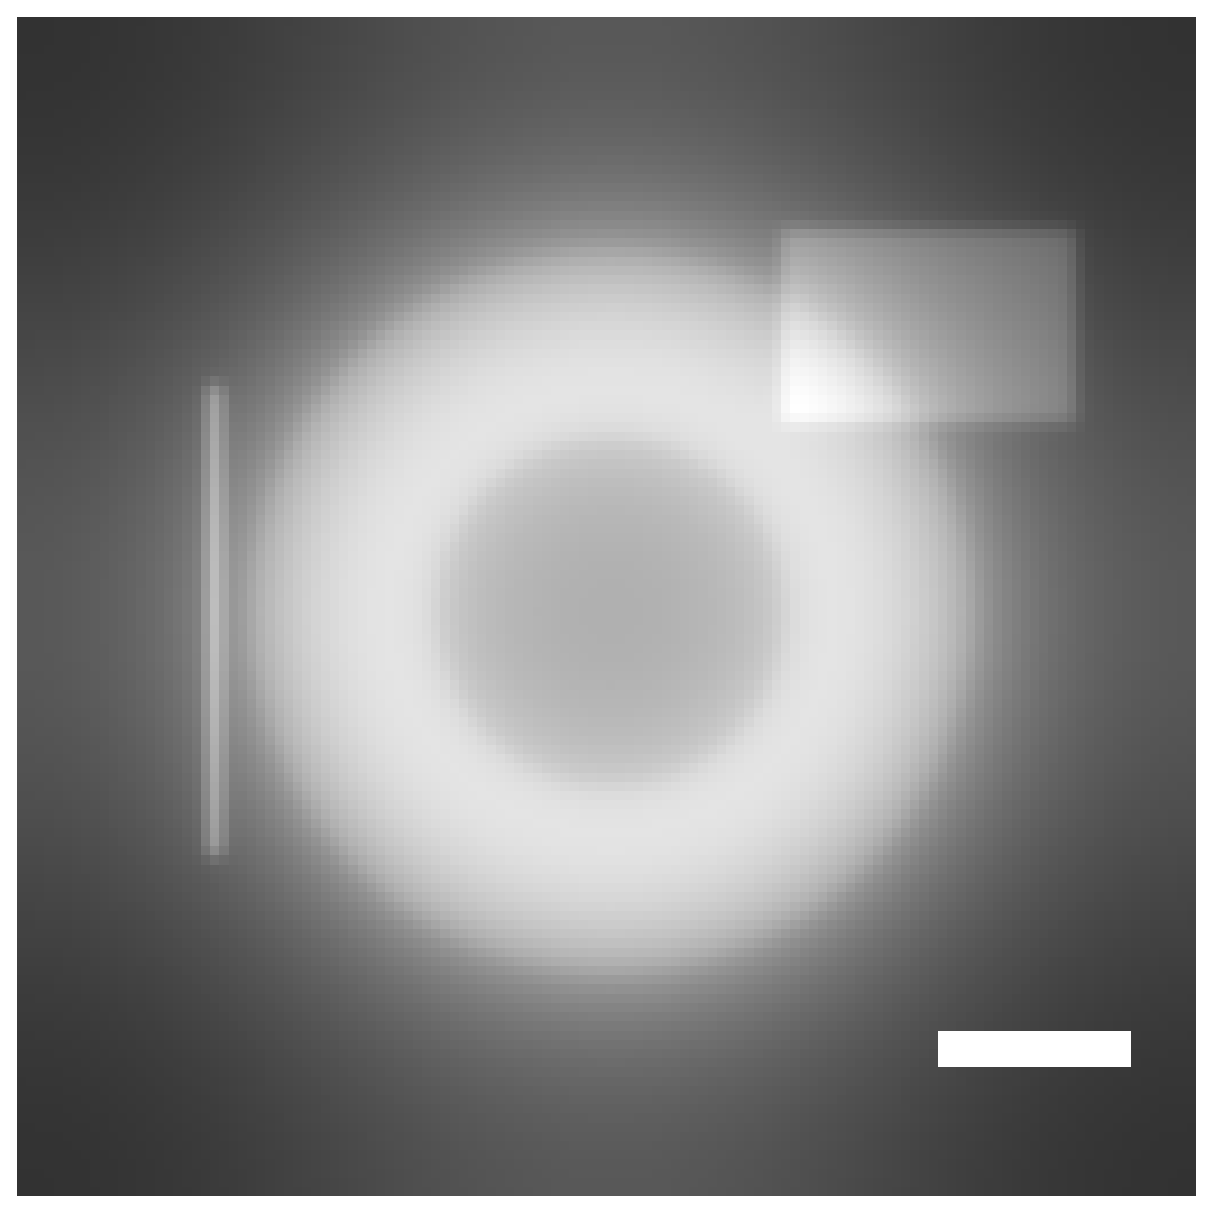
\includegraphics[width=4cm]{../app_hilo/iu}}
  \subfigure[image with structured illumination
  $I_n$]{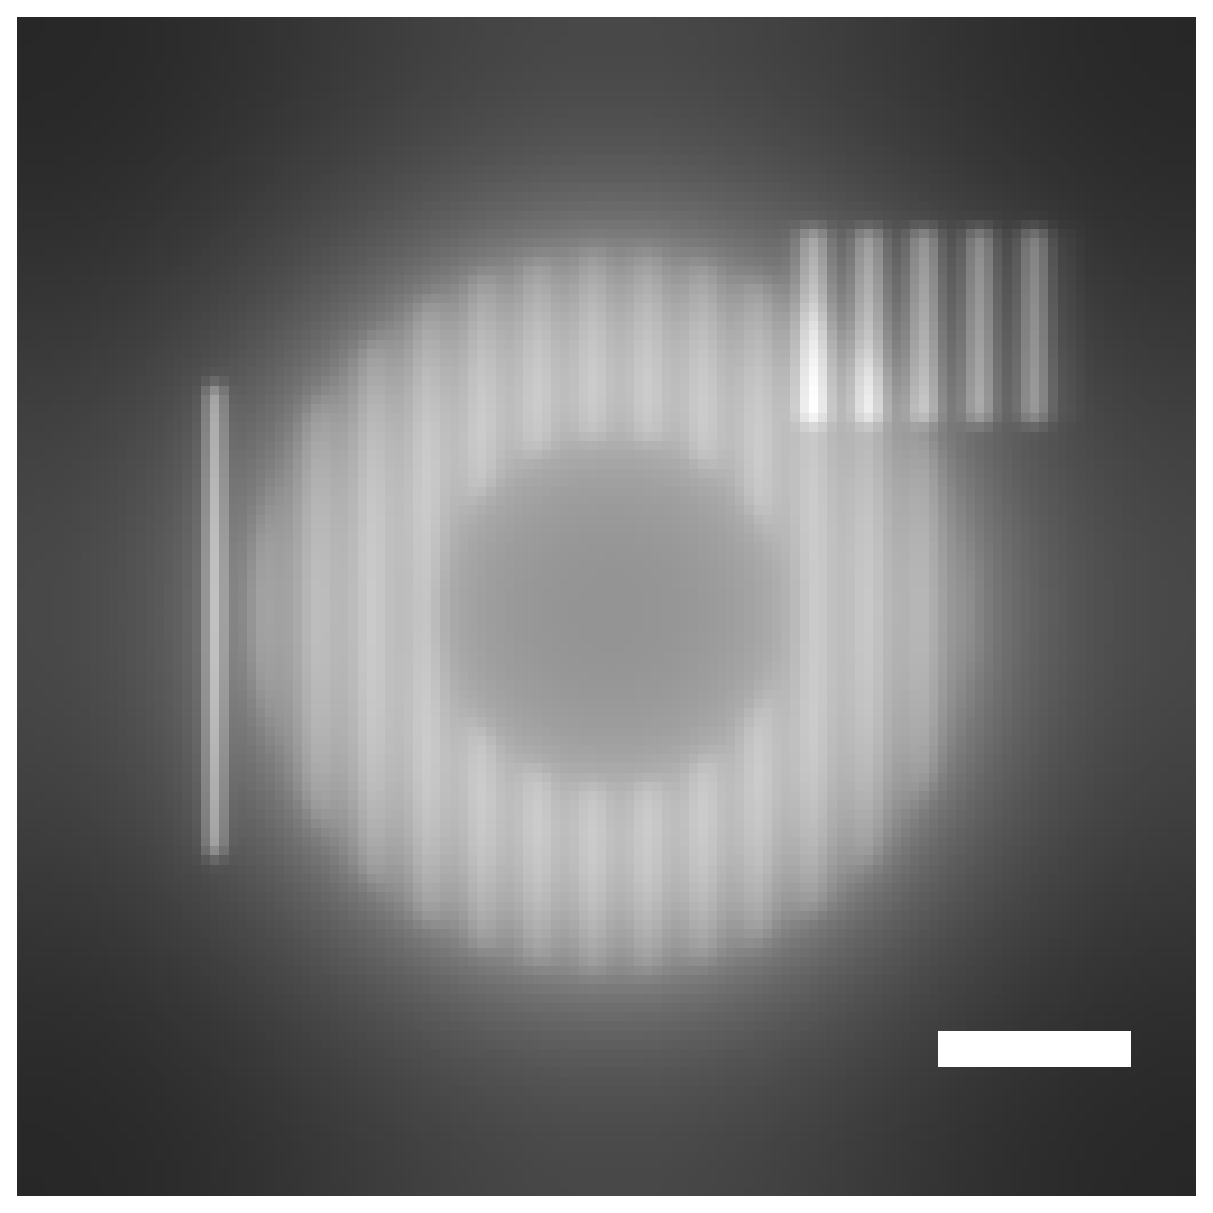
\includegraphics[width=4cm]{../app_hilo/in}}

  \caption{{\bf(a)} $xy-$slice of the object in the focal plane. It
    consists of a line, a spherical shell and a rectangle. Only the
    shell is extended in z. {\bf(b)} Image with widefield
    illumination. {\bf(c)} Image with structured illumination (grating
    period \unit[600]{nm}).  The scalebars are \unit[2]{$\mu$m}
    wide. }
  \label{fig:input}
\end{figure}
\figref{fig:defocus} shows the non-uniformly illuminated images for
different focus positions. The line and the rectangle both become
blurred and the contrast of the grating decreases in out-of-focus
planes. The grating in the sphere is still visible at approximately
the same contrast.
\begin{figure}[htb]
  \centering
  \subfigure[100 nm defocus]{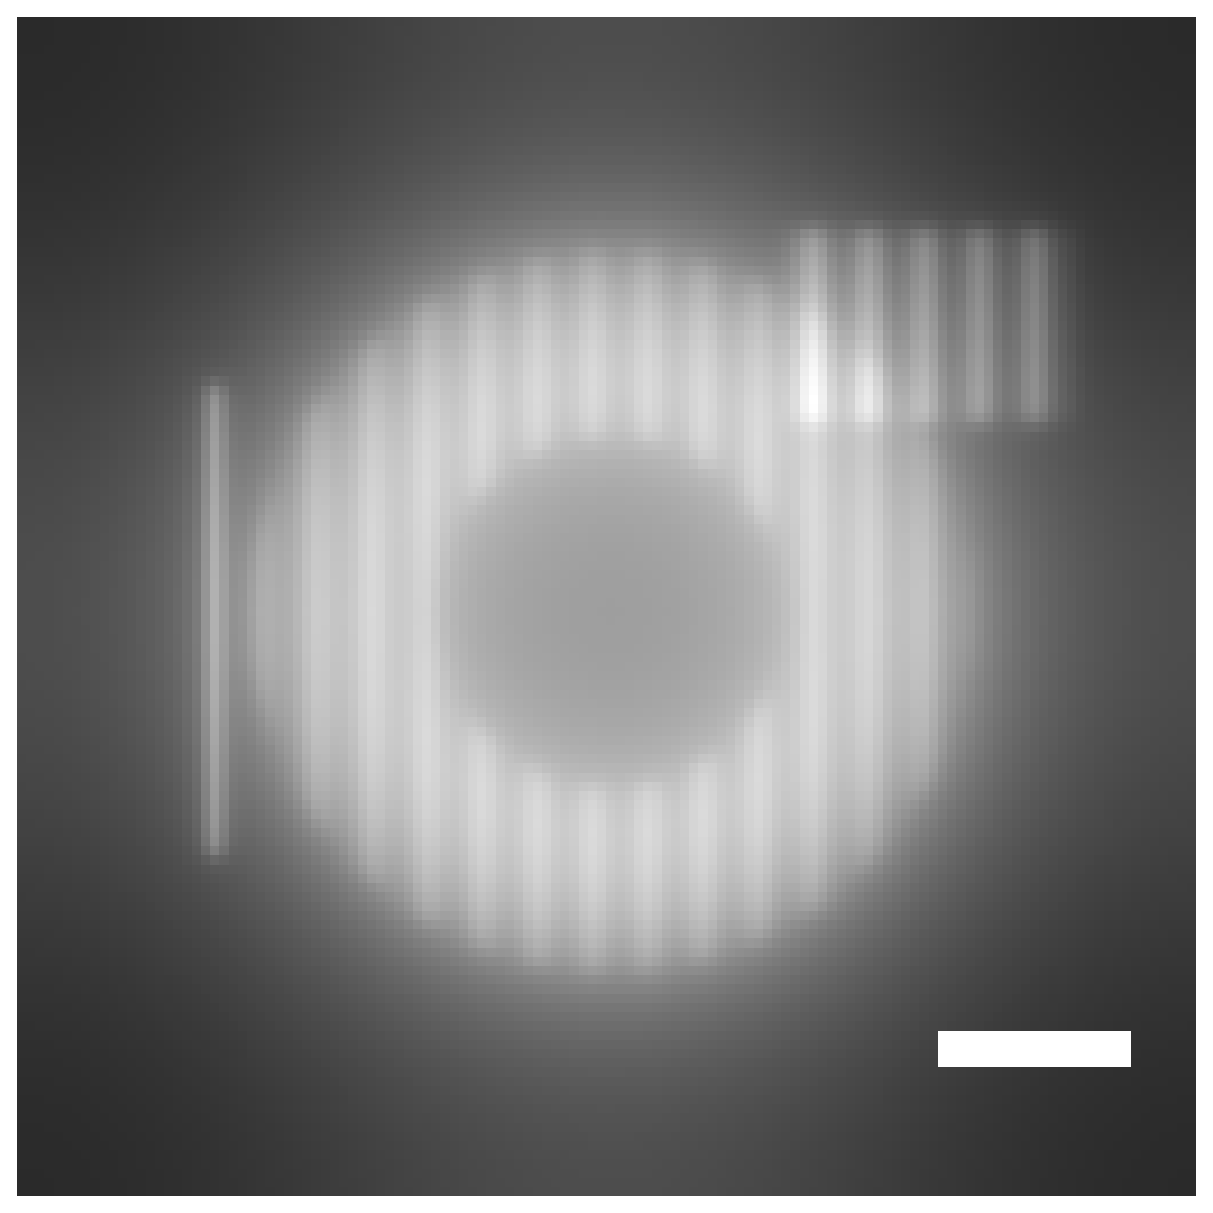
\includegraphics[width=4cm]{../app_hilo/in100}}
  \subfigure[200 nm]{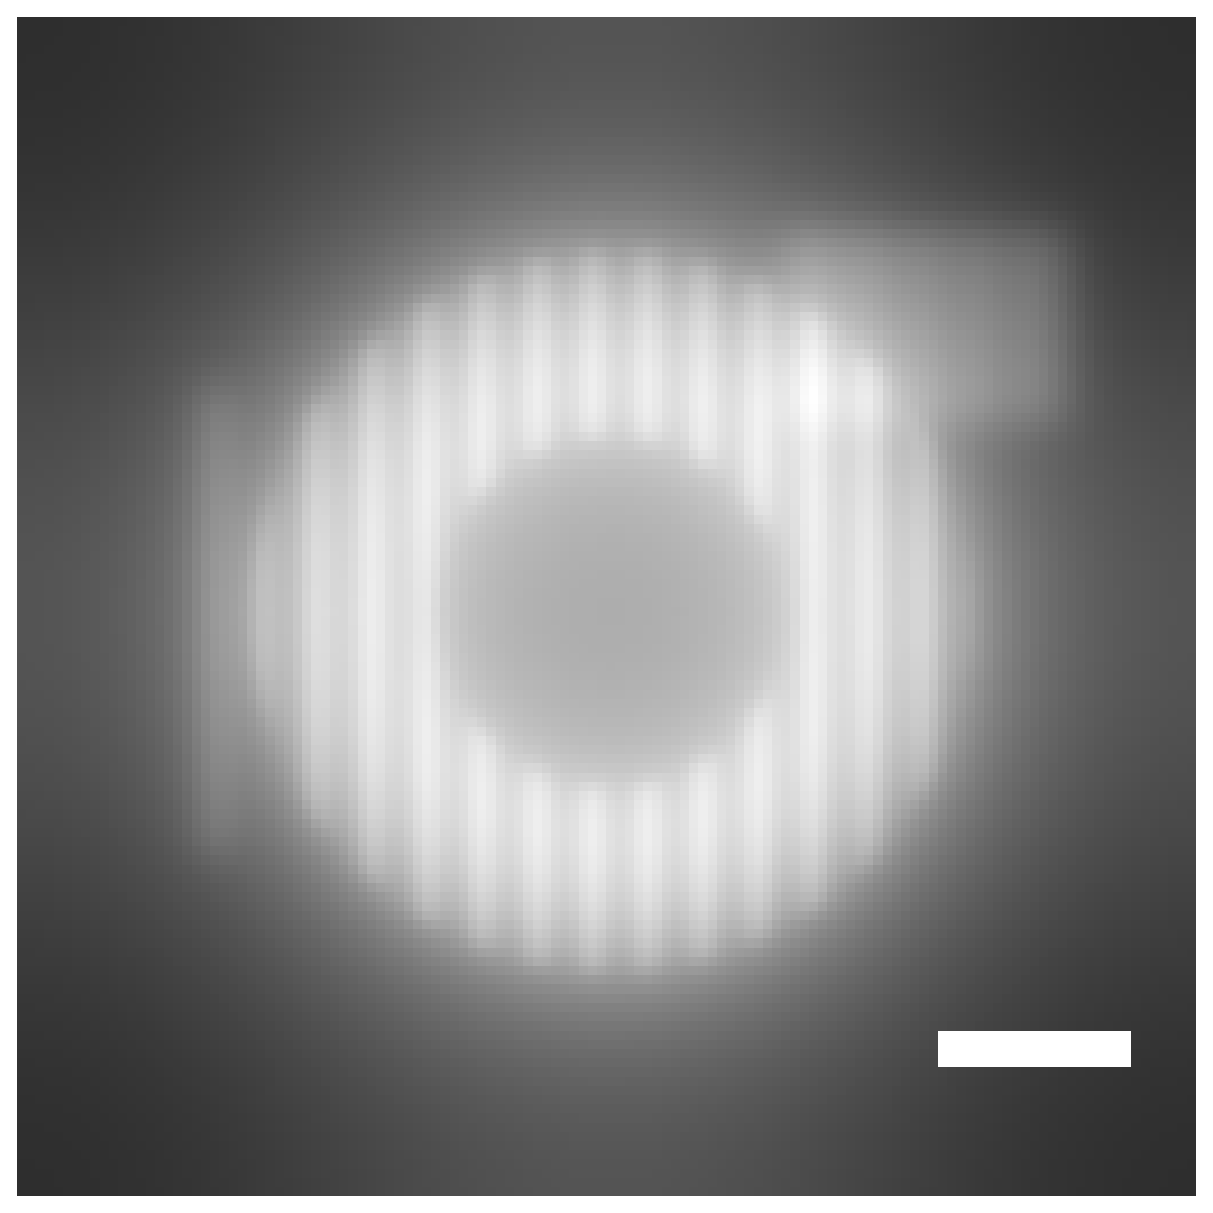
\includegraphics[width=4cm]{../app_hilo/in200}}
  \subfigure[500 nm]{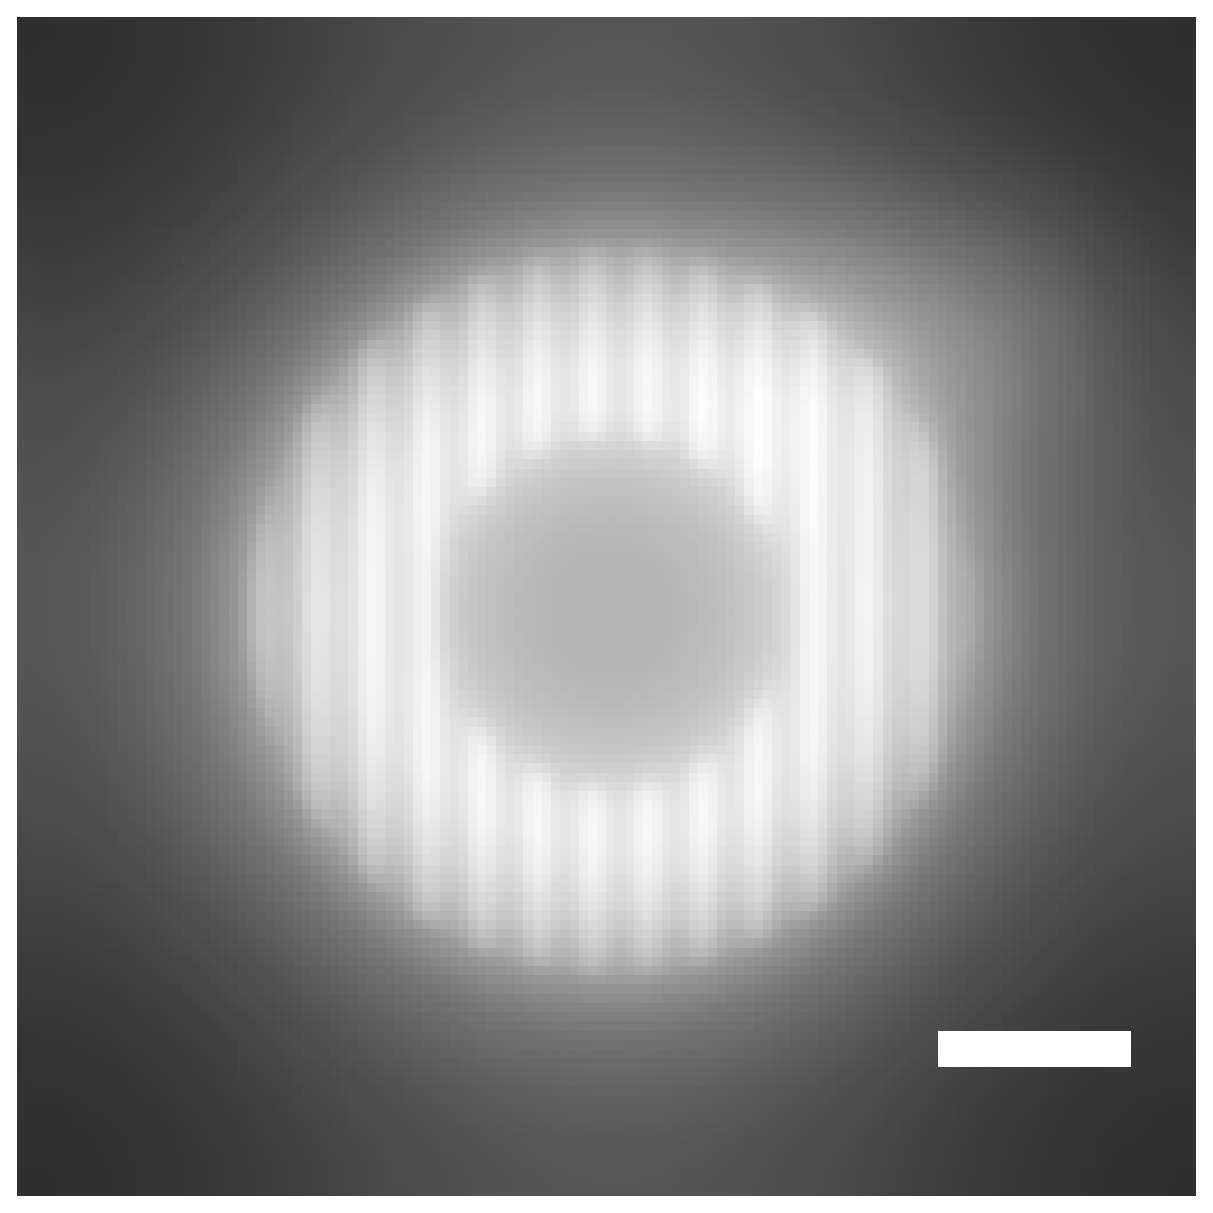
\includegraphics[width=4cm]{../app_hilo/in500}}
  \caption{Defocus series of the test object under structured coherent
    illumination (grating period \unit[600]{nm}). The scalebar is
    \unit[2]{$\mu$m} wide.}
  \label{fig:defocus}
\end{figure}
\section{Fundamentals of structured illumination}
If a fluorescent plane is imaged with a fluorescence widefield
microscope, the intensity of the image is constant no matter if the
plane is in focus or not (missing cone problem). 
\subsection{Apotome}
\label{sec:apotome}
Using non-uniform excitation light \cite{Neil1997} circumvent this
problem. They project a grid pattern into the sample using incoherent
illumination. For a fluorescent plane sample the modulation in the
image is highest, when the sample is in focus. If the plane is moved
out-of-focus, the modulation decreases. Hence it is possible to
achieve z-sectioning in a widefield microscope.

For one optically sectioned image $I_p$ they combine three grating
images $I_i$ (grating period
$1/\nu=\textrm{NA}/(\beta\lambda\tilde\nu)$, magnification $\beta$
between grating and specimen plane) with different phases:
\begin{align}
  I_p=\abs{I_1+I_2e^{i2\pi/3}+I_3e^{i4\pi/3}}
  \sim\left|2\frac{J_1(2u\tilde\nu(1-\tilde\nu/2))}{2u\tilde\nu(1-\tilde\nu/2)}\right|.
\end{align}

The last term is their result for the intensity of a fluorescent plane
with the defocus $u=8\pi z\sin^2(\alpha/2)/\lambda$. If no grating is
displayed ($\nu=0$) the resulting image $I_p$ is constant and the
microscope has no sectioning capability. A fine grating gives best
sectioning capability. However, there is also trade off to be made
because a fine grating will give very low contrast in a thick
specimen. Also for fine gratings a partially coherent illumination
should be used, so that orders are not cut off at the periphery of the
BFP \citetext{priv.\ comm.\ R.~Heintzmann}. This limits the field of
view for fine gratings.

For their reconstruction method it is necessary to capture three
images to compute one sectioned slice. This can be a problem if the
movement of the grating isn't perfect or if the object moves during
the exposures.
\subsection{HiLo}
This problem is addressed by \citet{2008Lim} and
\citet{2009Santos}. They describe an approach, for which only two
images need to be captured for each $z-$sectioned slice.  An image
with uniform illumination contains contributions of both in-focus and
out-of-focus fluorophores:
\begin{align}
\label{eqn:Iu}
  I_u(x,y)=I_\textrm{in}(x,y)+I_\textrm{out}(x,y).
\end{align}
The contribution from out-of-focus light $I_\textrm{out}$ is limited
to low spatial frequencies, i.e. $\tilde I_\textrm{out}(k_x,k_y)$ has
small support. The modulated part of the non-uniformly illuminated
image $I_n$ contains only information of the in-focus object
structure:
\begin{align}
\label{eqn:In}
  I_n(x,y)&=I_\textrm{in}(x,y)(1+M
  \sin(\kappa x+\varphi))+I_\textrm{out}(x,y),\\
  \kappa&=\frac{2\pi}{\lambda}n\sin(\alpha)\nu.
\end{align}
We can recover the sectioned image as a combination of high-frequency
components of the widefield image $I_u$ and the low-frequency
components of the modulated part of the non-uniform image $I_n$.
\subsubsection{Using speckle pattern as non-uniform illumination (local variance estimation)}
In the older publication \citep{2008Lim} a random speckle pattern is
projected into the sample. For comparison with the other methods we
describe a reimplementation of their method.

In order to process the non-uniform image it is divided into
subregions.  As a measure of local contrast in each of these
subregions the relative standard deviation $c$ is calculated (the
operator $\avg{\cdot}$ indicates averaging over a pixel
neighbourhood):
\begin{align}
  c_n=\frac{\sqrt{\avg{I_n^2}-\avg{I_n}^2}}{\avg{I_n}}.
\end{align}
The relative standard deviation $c_n$ will be zero for image regions
without in-focus contributions. Its value increases as the modulation
of the non-uniform illumination increases (that's what we
want). However $c_n$ also increases if there is a small in-focus
feature. In that we are not interested as we only want to build up an
image of in-focus fluorophores with low spatial frequencies. 

The authors state that a corrected relative standard deviation $c_s$
of the non-uniform illumination can be obtained by removing the
standard deviation
$c_0=\frac{\sqrt{\avg{I_u^2}-\avg{I_u}^2}}{\avg{I_u}}$ of the
widefield image:
\begin{align} 
  c_s^2=\frac{c_n^2-c_0^2}{1+c_0^2}
  =
  \frac{\avg{I_n^2}}{\avg{I_n}^2}
  \frac{\avg{I_u^2}}{\avg{I_u}^2}-1.
\end{align}
The product $I_{su}=c_s\avg{I_u}$ then provides a low resolution
version of $I_u$ that is optically sectioned (using information from
$I_n$) even for the DC frequency.

The following listing shows how this algorithm can be applied to two
input images {\sf iu} and {\sf in}. Instead of doing a discrete
integration over regions we multiply with a Gaussian in Fourier
space. The cutoff frequency $k_c$ of the filter is chosen low enough
so that $c_s$ doesn't contain any structure of the grating anymore.
\begin{lstlisting}
si=size(in);   n=si(1);  % only square images
kc=0.04;                 % filter cutoff
r=rr(in,'freq');
klp=exp(-r.^2/(2*kc^2)); % low pass
khp=1-klp;               % high pass
ina=ift(ft(in).*klp);
in2a=ift(ft(in.^2).*klp);
iua=ift(ft(iu).*klp);
iu2a=ift(ft(iu.^2).*klp);
cs2=in2a.*iua.^2./(ina.^2.*iu2a)-1;
isu=sqrt(cs2).*iua;      % sectioned version of iu
kihp=ft(iu).*khp;
kilp=ft(isu).*klp;
\end{lstlisting}
\begin{figure}[htb]
  \centering
  \subfigure[Corrected relative standard deviation $c_s$.]{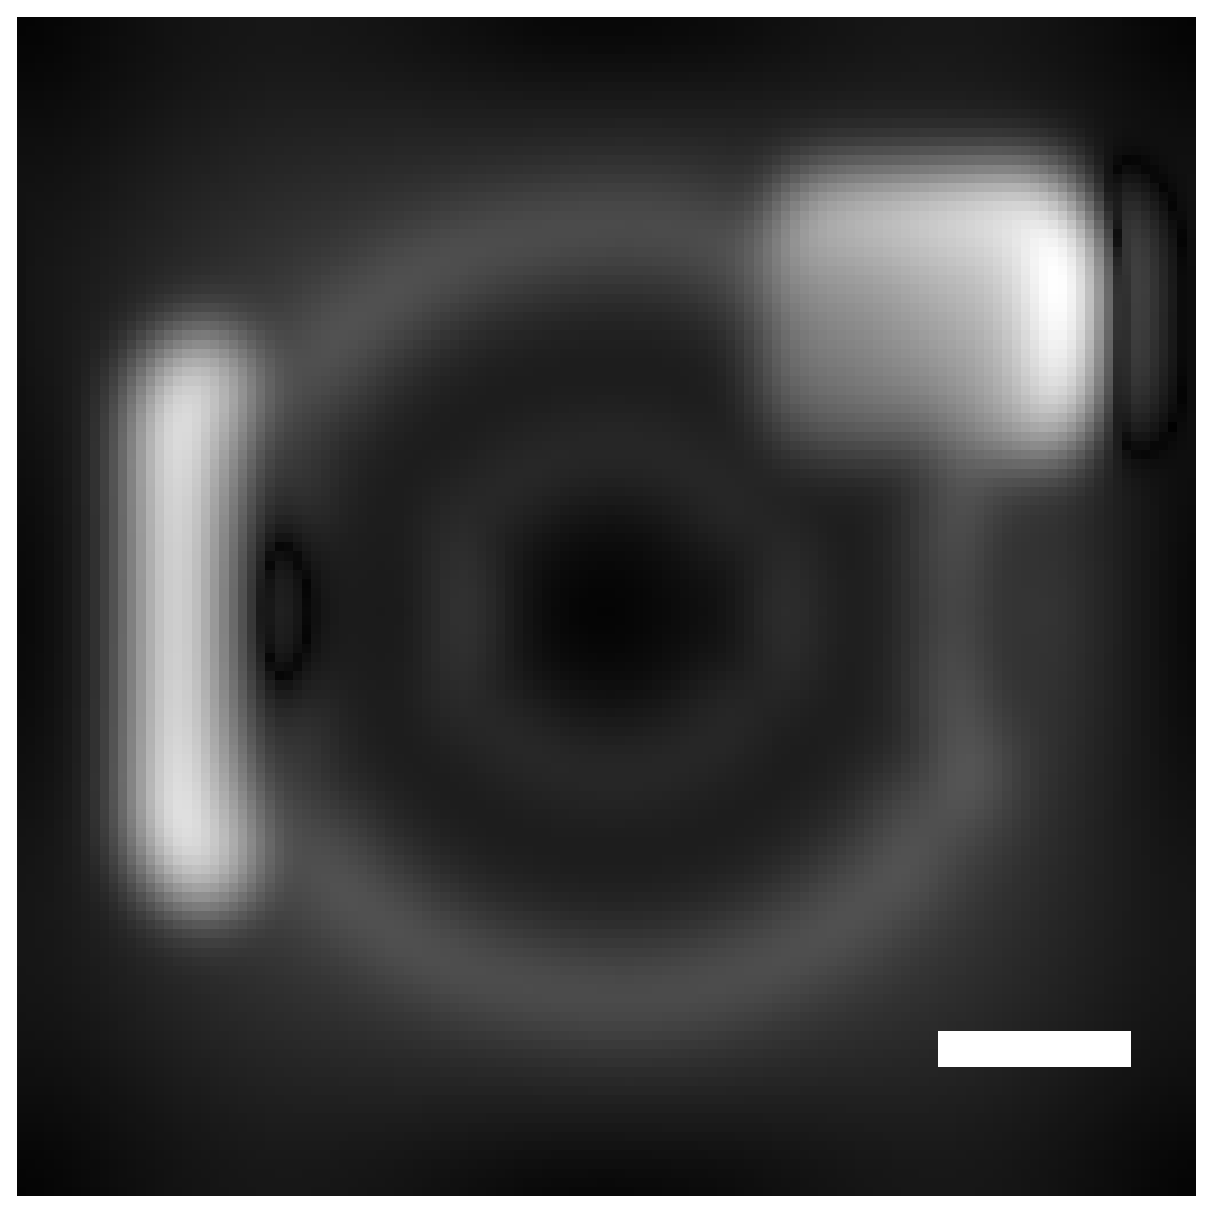
\includegraphics[width=4cm]{../app_hilo/cs}}
  \subfigure[The product $I_{su}=c_sI_u$]{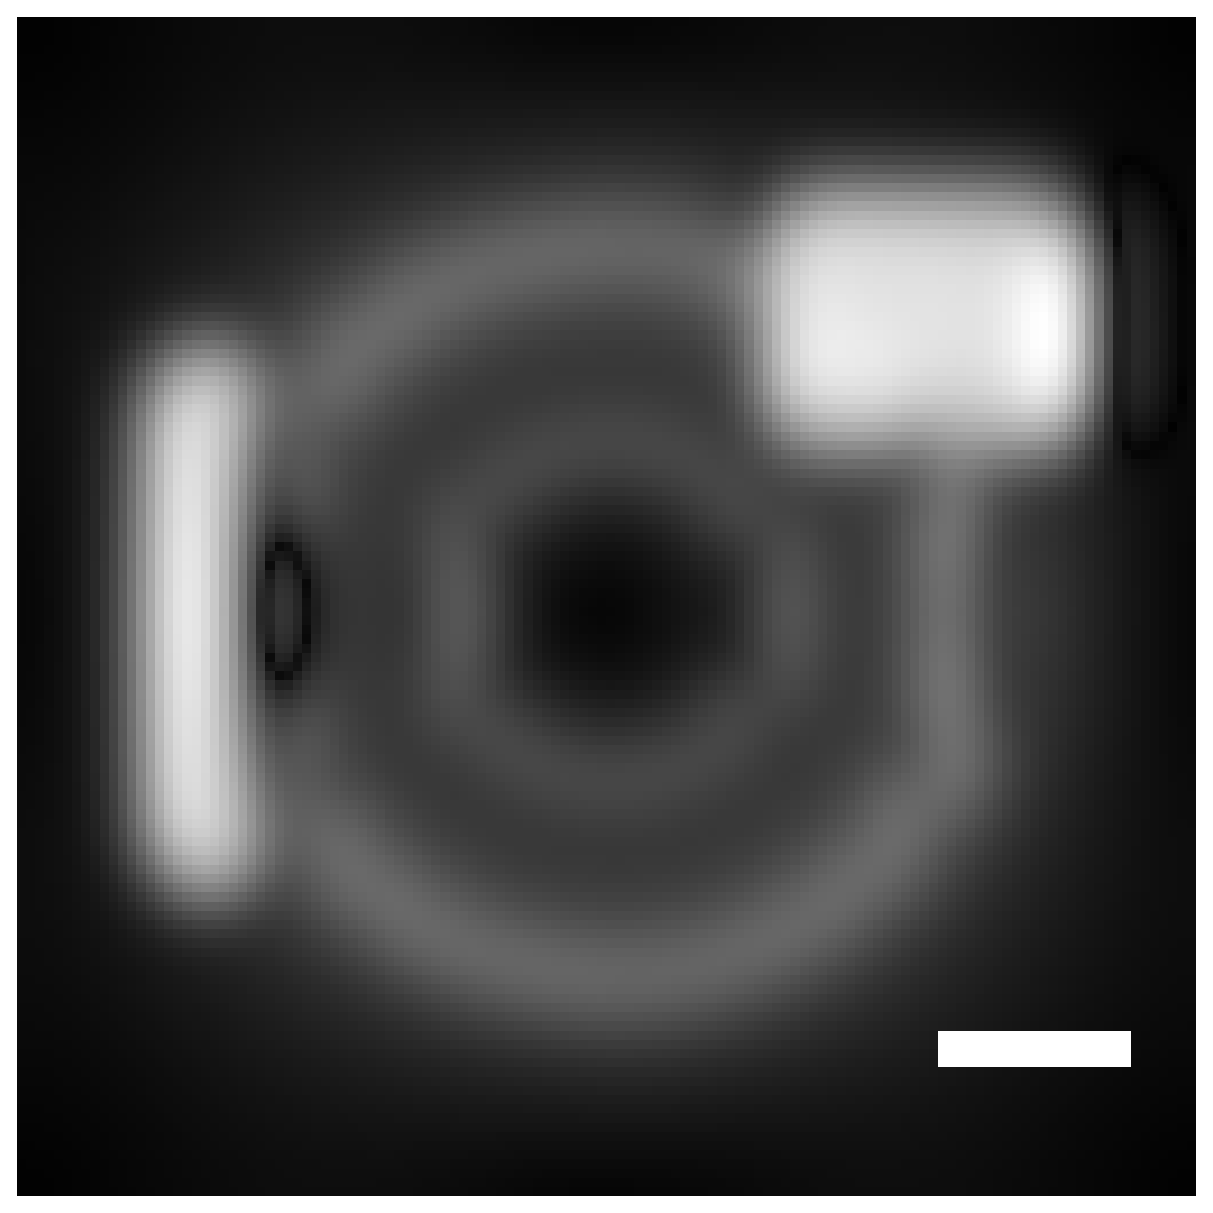
\includegraphics[width=4cm]{../app_hilo/isu}}
  \subfigure[Low spatial frequency section $I_\textrm{lp}$]{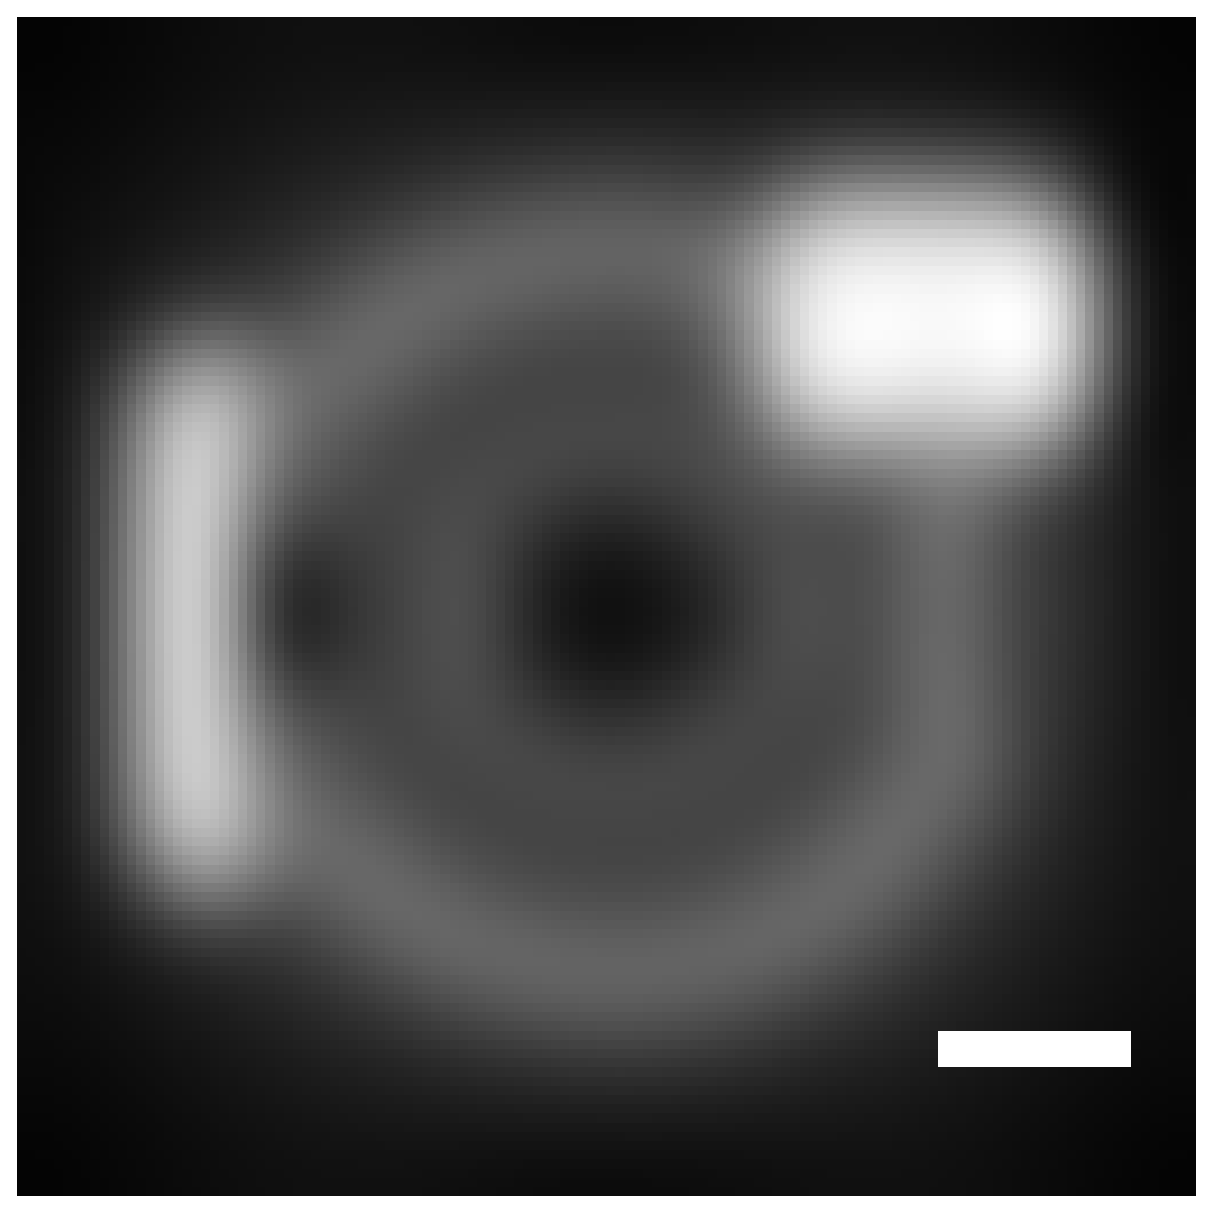
\includegraphics[width=4cm]{../app_hilo/ilp}}
  \caption{Several intermediate results of the algorithm. The scalebar is
    \unit[2]{$\mu$m} wide.}
  \label{fig:hilo1interm}
\end{figure}
The HiLo method combines a low-pass filtered version of $I_{su}$ with
a high pass filtered version of the uniformly illuminated image $I_u$.
To do this the two images are scaled for a seamless interface along
the circle $K$ with radius $\abs{\vect k_c}$ in k-space and then added:
\begin{align}
  \eta=\!\!\!\!\ointop_{\partial K_{k_c}}\!\!\!
  \frac{\abs{I_\textrm{hp}}}{\abs{I_\textrm{lp}}}\,\textrm{d}\vect k,\\
  I_\textrm{hilo}=\eta I_\textrm{lp}+I_\textrm{hp}.
\end{align}

This is done in the following listing:
\begin{lstlisting}
ring=real(ft(besselj(0,2*pi*kc*n.*r)));
ring2=r-1./n<kc & r+1./n>kc;
cring=ring.*ring2;
nring=cring./sum(cring); % normalized ring with radius kc
eta=sum(abs(kihp)./abs(kilp).*nring);
ihilo=ift(eta.*kilp+kihp);
\end{lstlisting}

\begin{figure}[htb]
  \centering
  \subfigure[High frequency components $I_\textrm{hp}$ of widefield.]{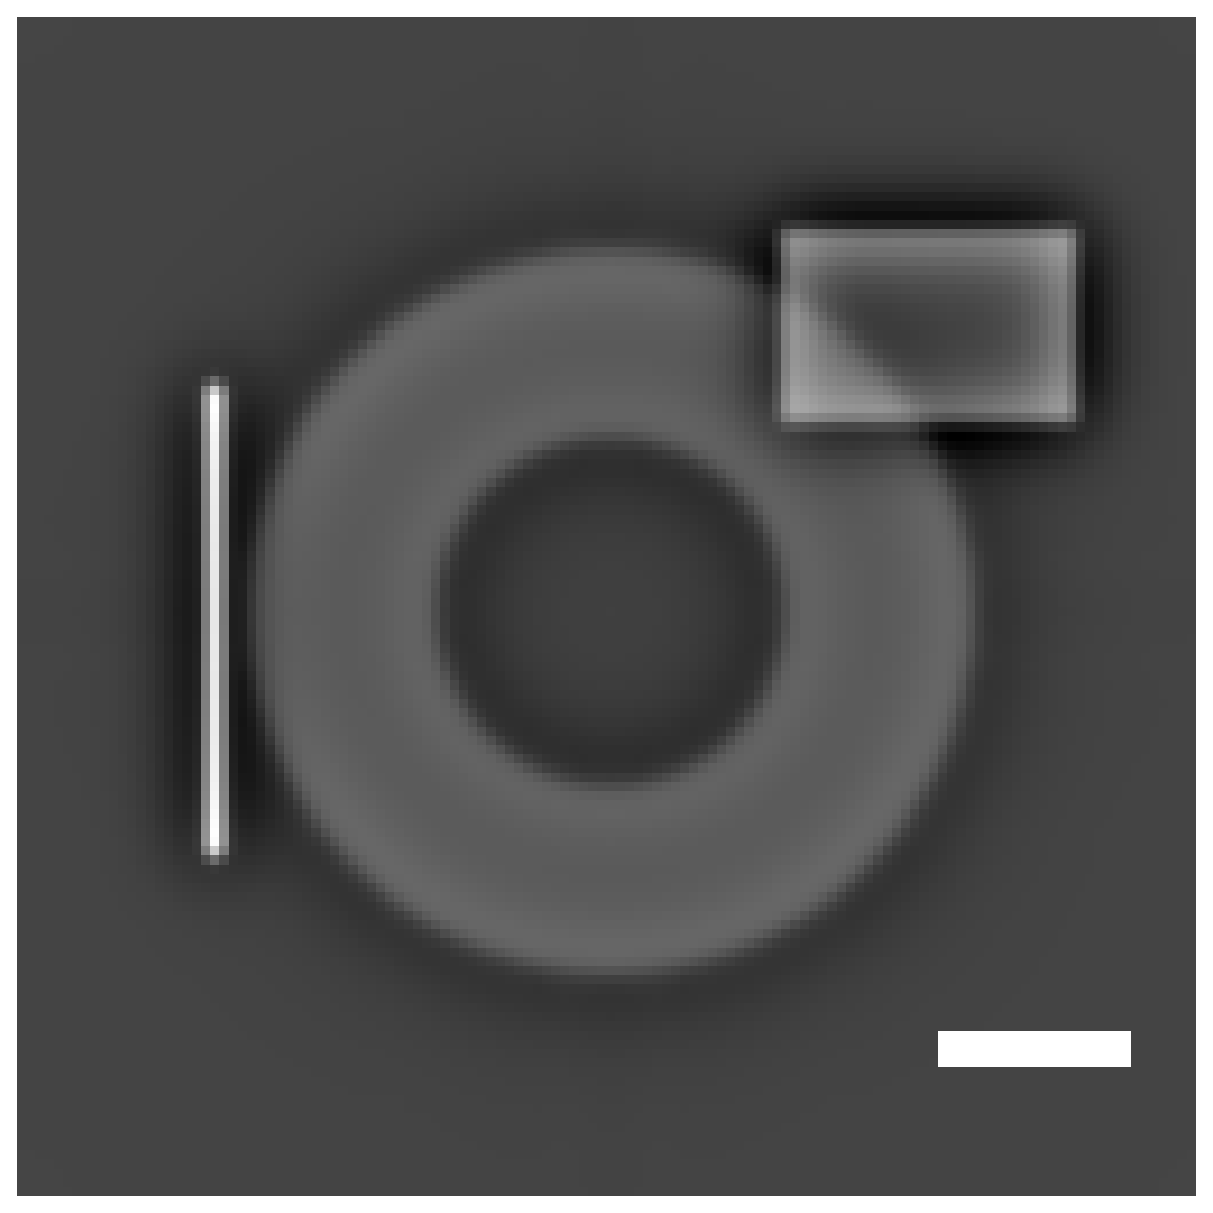
\includegraphics[width=4cm]{../app_hilo/ihp}}
  \subfigure[Combined images $\tilde I_\textrm{hilo}$ in k-space.]{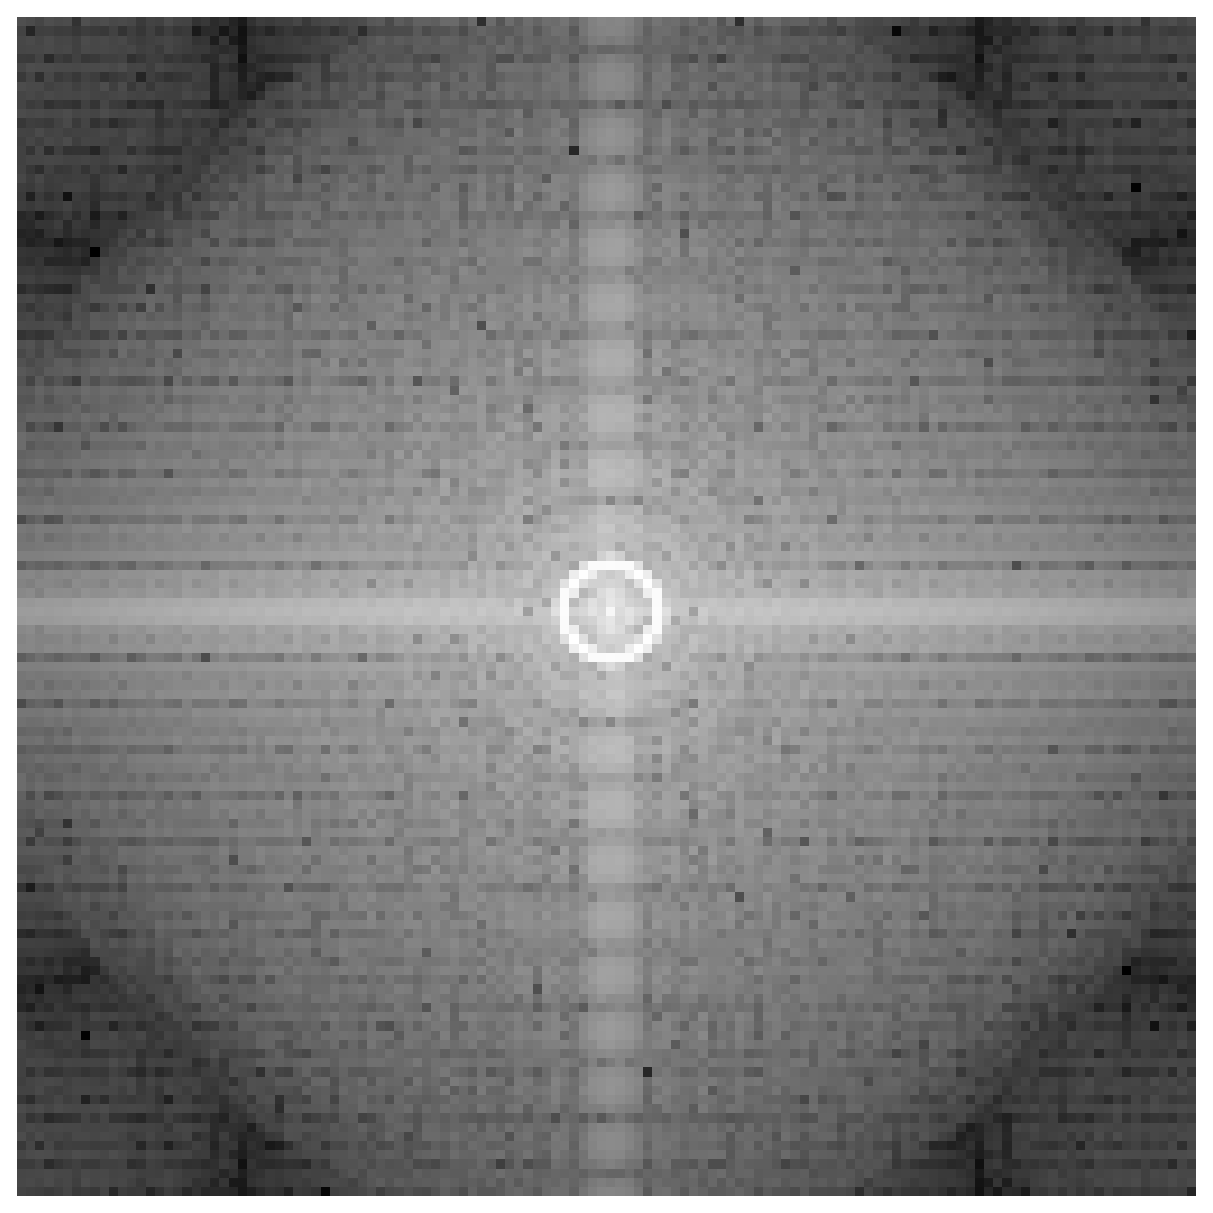
\includegraphics[width=4cm]{../app_hilo/kihilo}}
  \subfigure[Combined section $I_\textrm{hilo}$.]{\label{fig:ihilo}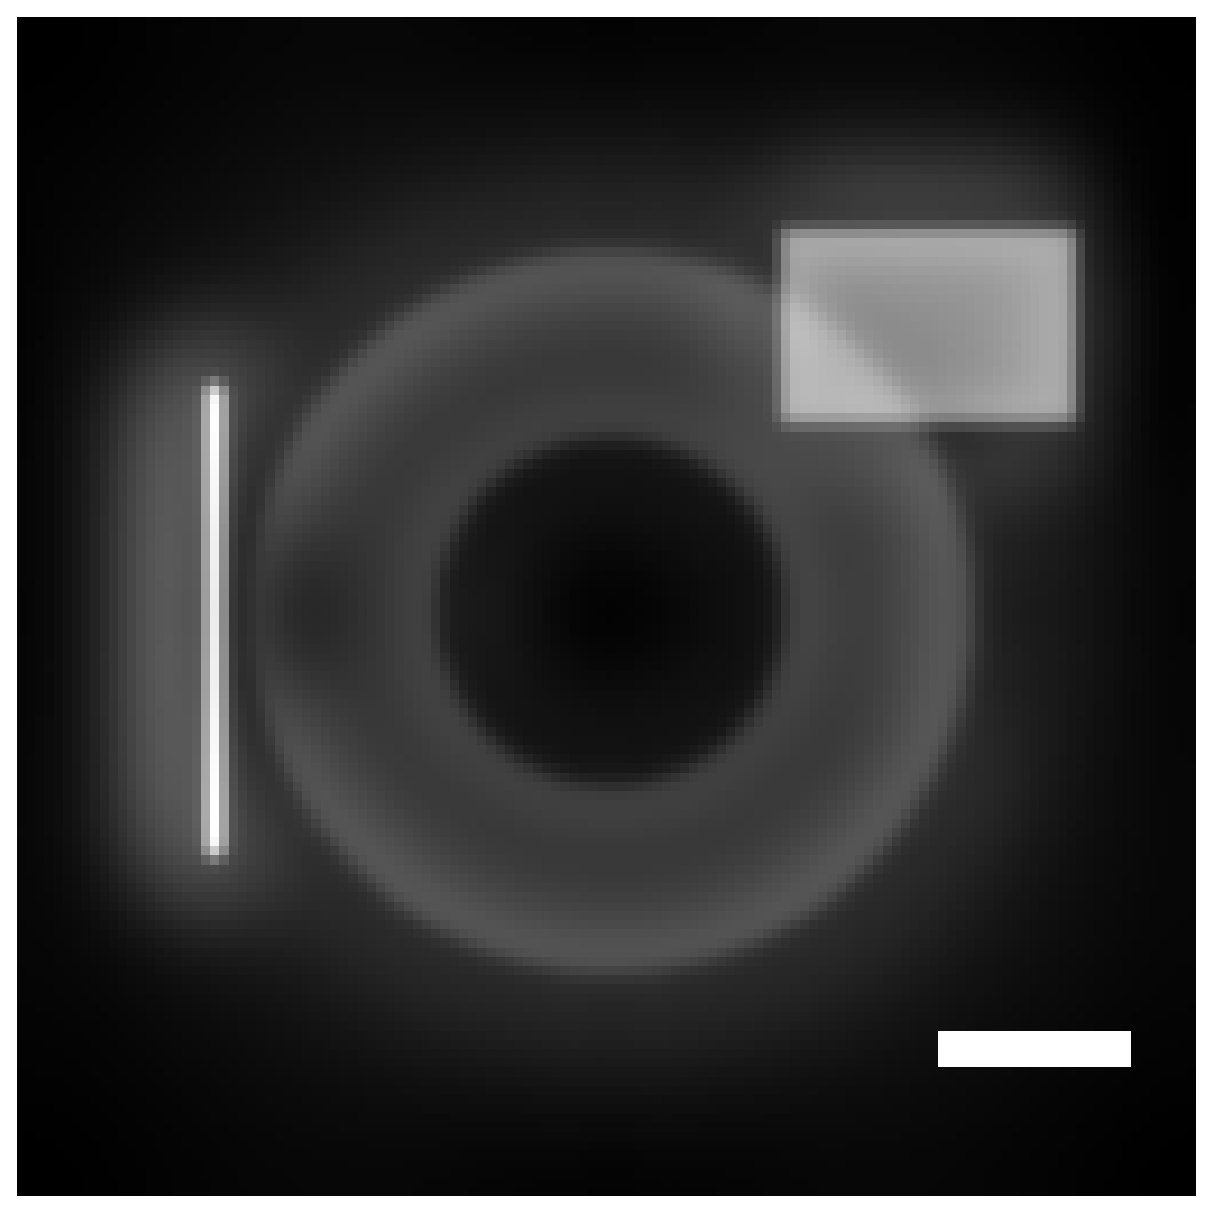
\includegraphics[width=4cm]{../app_hilo/ihilo}}
  \caption{More intermediate and the end result of the HiLo local
    variance estimation algorithm. The white circle in image {\bf (b)}
    marks the cutoff frequency $k_c$ of the spatial low pass
    filter. The scalebars are \unit[2]{$\mu$m} wide.}
  \label{fig:hilo1interm2}
\end{figure}

\subsubsection*{Discussion}
This algorithm only requires the illumination intensity in $I_n$ to
fluctuate over a certain region and one uniform image. The
reconstructed results somewhat resemble a sectioned image. The main
advantage is that all the filtering could have been done in real
space, without ever doing any Fourier transform.
\subsubsection{Reconstructing the sample illuminated with a grating
  pattern (single side-band demodulation)}
The more recent paper \cite{2009Santos} uses a more defined pattern in
the excitation illumination than random speckle. A grating is
projected into the specimen using a spatial light modulator.

Starting from a widefield image $I_u$ and an image $I_n$ that has been
illuminated with a grating they first determine the ratio $R=I_n/I_u$.
With equations \eqref{eqn:Iu} and \eqref{eqn:In} defining the
relationship between in-focus and out-of-focus light in both images
they obtain:
\begin{align}
  R&=1+CM\sin(\kappa x+\varphi)),\\
  C&=\frac{I_\textrm{in}}{I_\textrm{in}-I_\textrm{out}}.
\end{align}
Here $C$ is the local image contrast (containing information similar
to $c_s$ in the HiLo local variance method) that is necessary to
determine the low-resolution sectioned image. The Fourier transform
$\tilde R$ (see \figref{fig:hatR}) of the ratio contains a peak in the
centre (due to the constant 1). Then there are strong $\pm 1$ orders
and weaker $\pm 2$ orders because a rectangular grating is imaged into
the sample. If only a Sine grating was imaged into the sample, only the $\pm 1$ orders would be present.
%FIXME the weak grating isn't in In! so maybe it is due to the ratio

To extract the modulated signal from $R$, a filter is constructed that
selects only the first order on the right side of the Fourier
transform $\tilde R$. The result of the filter is shown in
\figref{fig:hatR+}. The intermediate image $I_{su}=\abs{R^+}I_u$ (see
\figref{fig:isu2}) contains the low-resolution sectioned image.

\begin{figure}[htb]
  \centering \subfigure[Ratio
  $R=I_n/I_u$.]{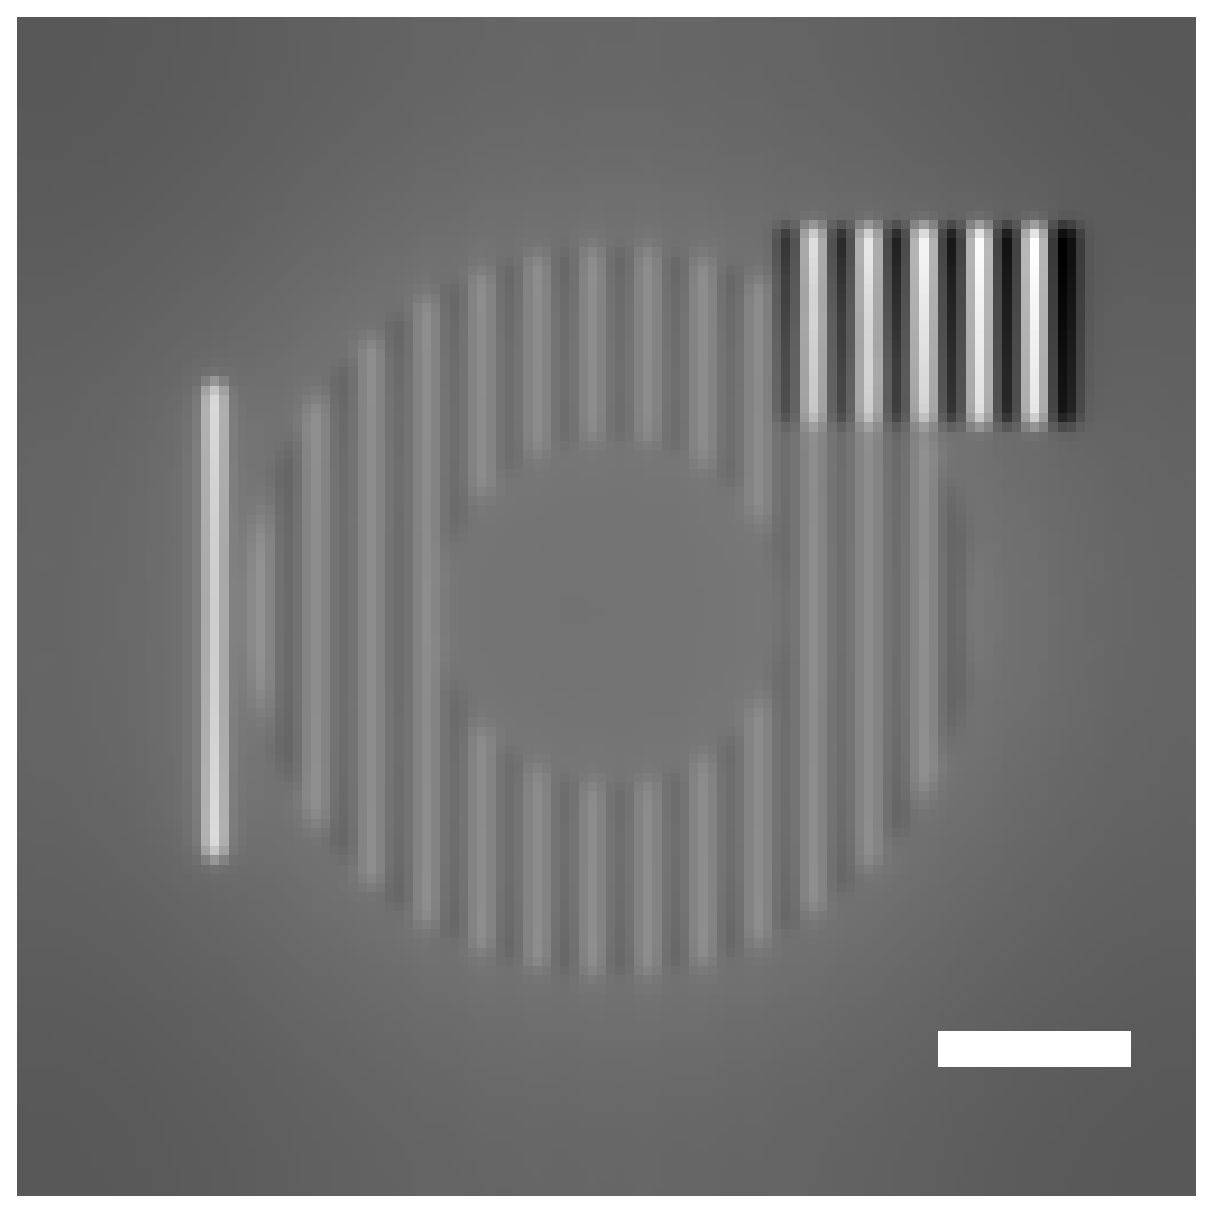
\includegraphics[width=4cm]{../app_hilo/ratio}}
  \subfigure[Fourier transform $\tilde
  R$.]{\label{fig:hatR}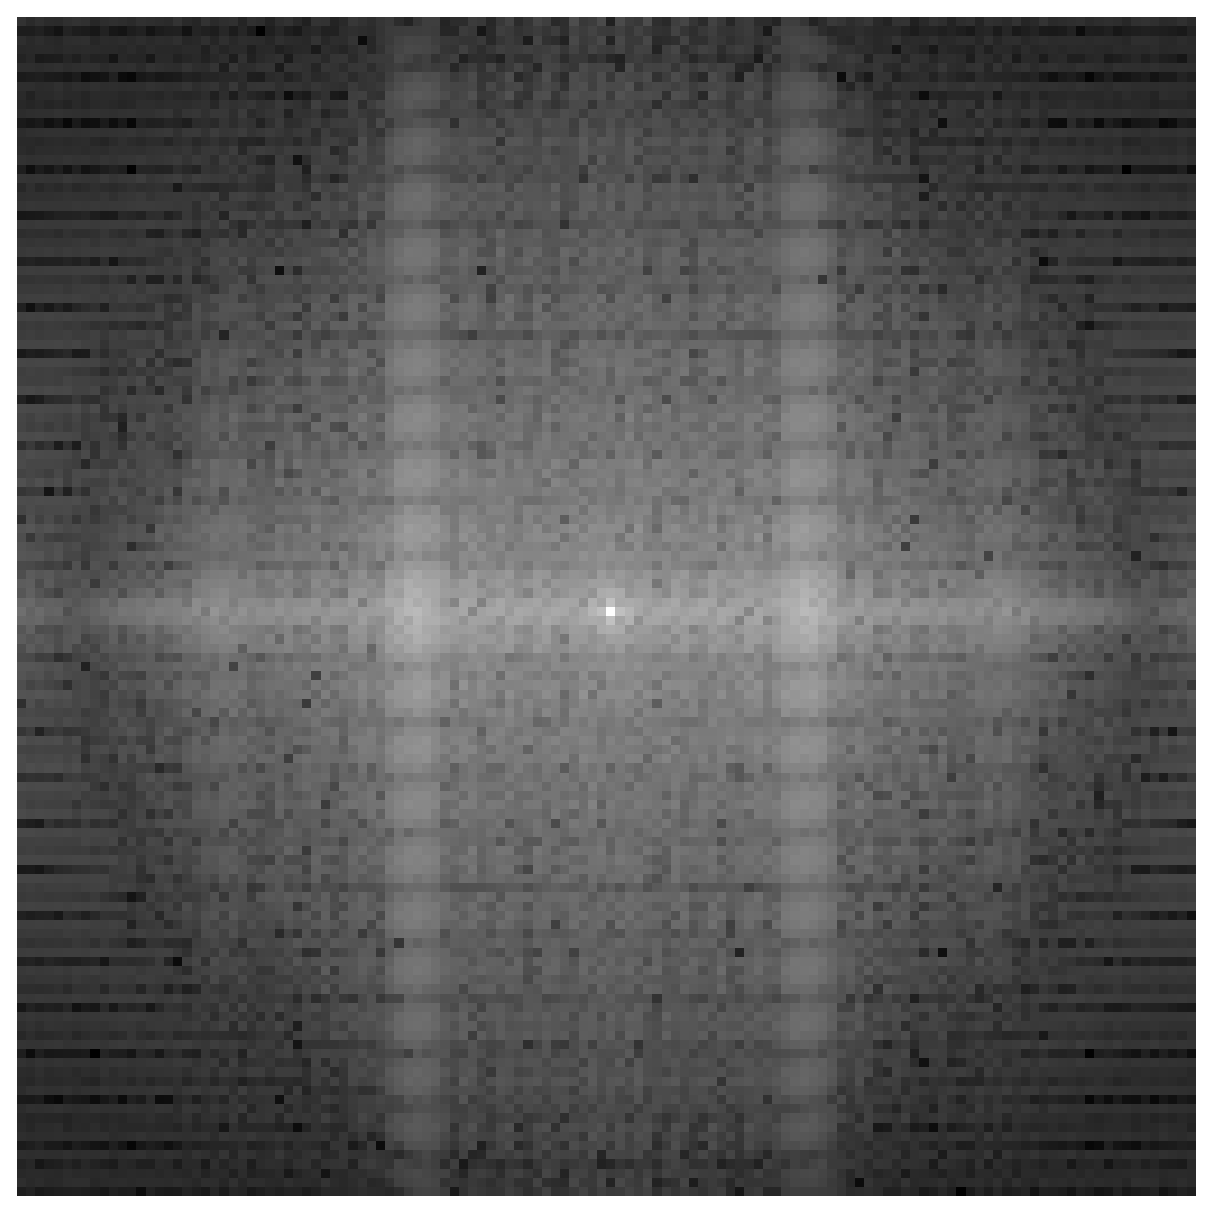
\includegraphics[width=4cm]{../app_hilo/ftratio}}
  \subfigure[Filtered first order $\tilde
  R^+$.]{\label{fig:hatR+}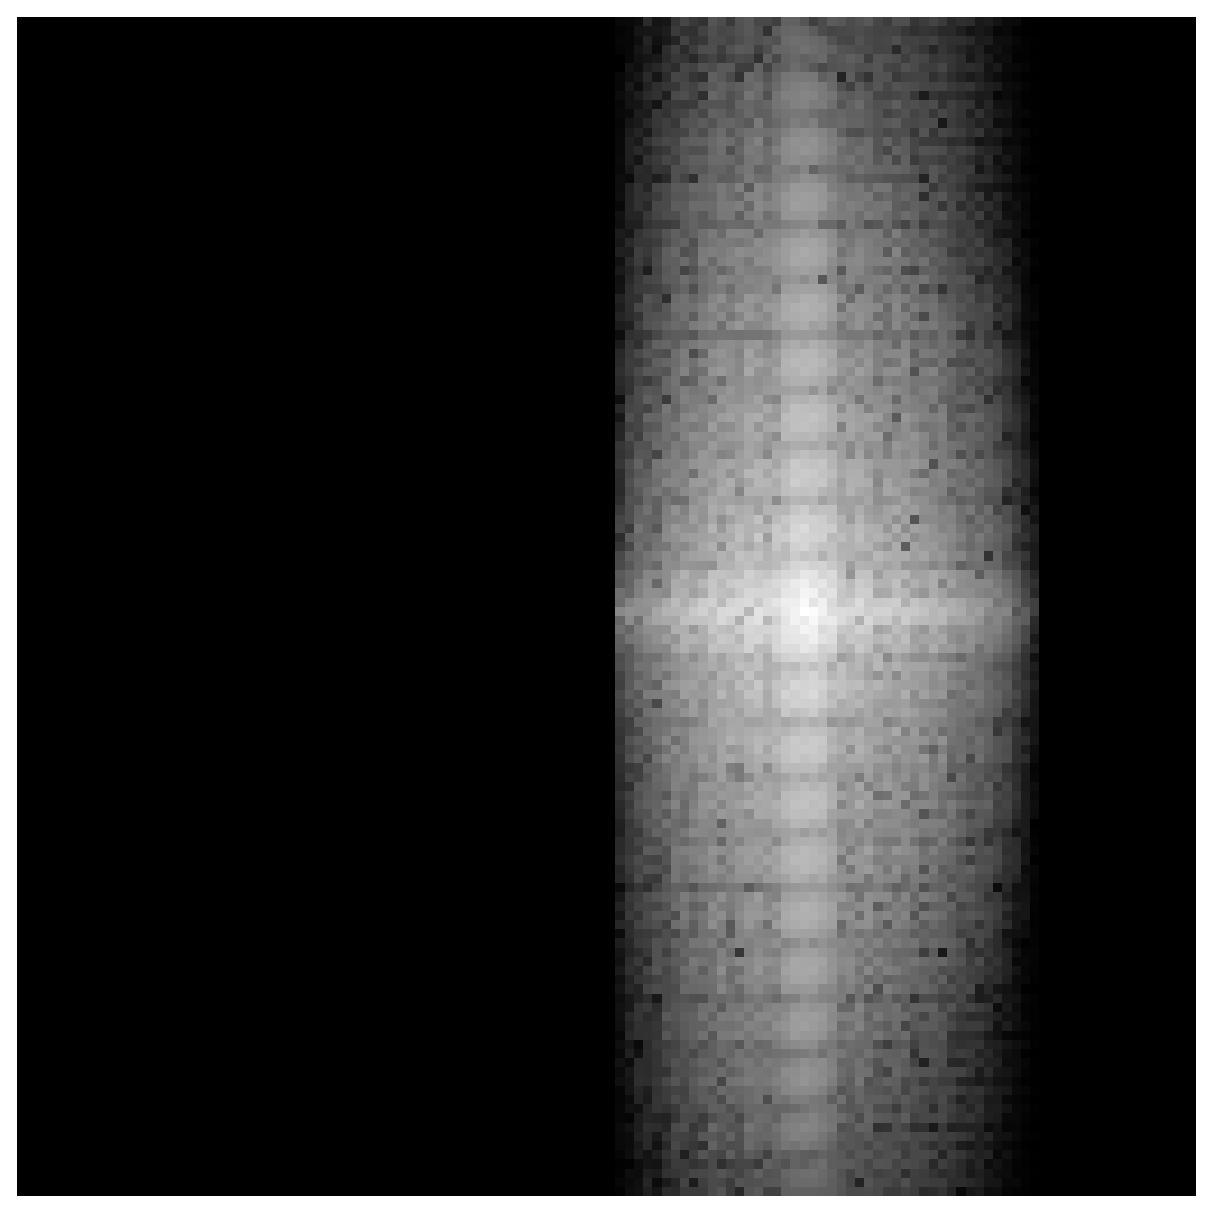
\includegraphics[width=4cm]{../app_hilo/filterftratio}}
  \caption{Intermediate results for the HiLo single side-band
    demodulation algorithm. The scalebar in (a) is \unit[2]{$\mu$m}
    wide.}
  \label{fig:hilo2}
\end{figure}

The following listing shows the code for the algorithm:
\begin{lstlisting}
si=size(in);   n=si(1);   r=rr(in,'freq');
ratio=in./iu;
%% select R+ and construct isu
filter=gaussf((xx(in,'freq')>0.1) & (xx(in,'freq')<0.27),4);
ftratio=ft(ratio);
cm=abs(ift(filter.*ftratio));
isu=cm.*iu
kc=.07;          % calculate low pass filtered low-res section
klp=exp(-r.^2/(2*kc^2));
ilp=real(ift(klp.*ft(isu)))
% calculate high pass filtered high-res section
ihp=real(ift((1-klp).*ft(iu)))
% construct the circle for integration in k-space
ring=abs(ft(besselj(0,2*pi*kc*n.*r)));
ring2=r-1./n<kc & r+1./n>kc;
cring=ring.*ring2;
nring=cring./sum(abs(cring))
eta=sum(abs(ft(ihp))/abs(ft(ilp)).*nring) % integrate along circle
ihilo=eta.*ilp+ihp                        % combined section
\end{lstlisting}
We chose the cutoff frequency $k_c$ high enough so that the low
resolution sectioned image $I_\textrm{lp}$ (computed from uniform
image) doesn't look too smooth but also low enough so that not too
much information is lost from the high resolution sectioned image
$I_\textrm{hp}$ image (computed from modulated image). The scale
factor $\eta$ for $I_\textrm{lp}$ and $I_\textrm{hp}$ is calculated as
in the previous section. Finally the combined sectioned image is
displayed in \figref{fig:ihilo2}.
\begin{figure}[htb]
  \centering
  \subfigure[$I_{su}$]{\label{fig:isu2}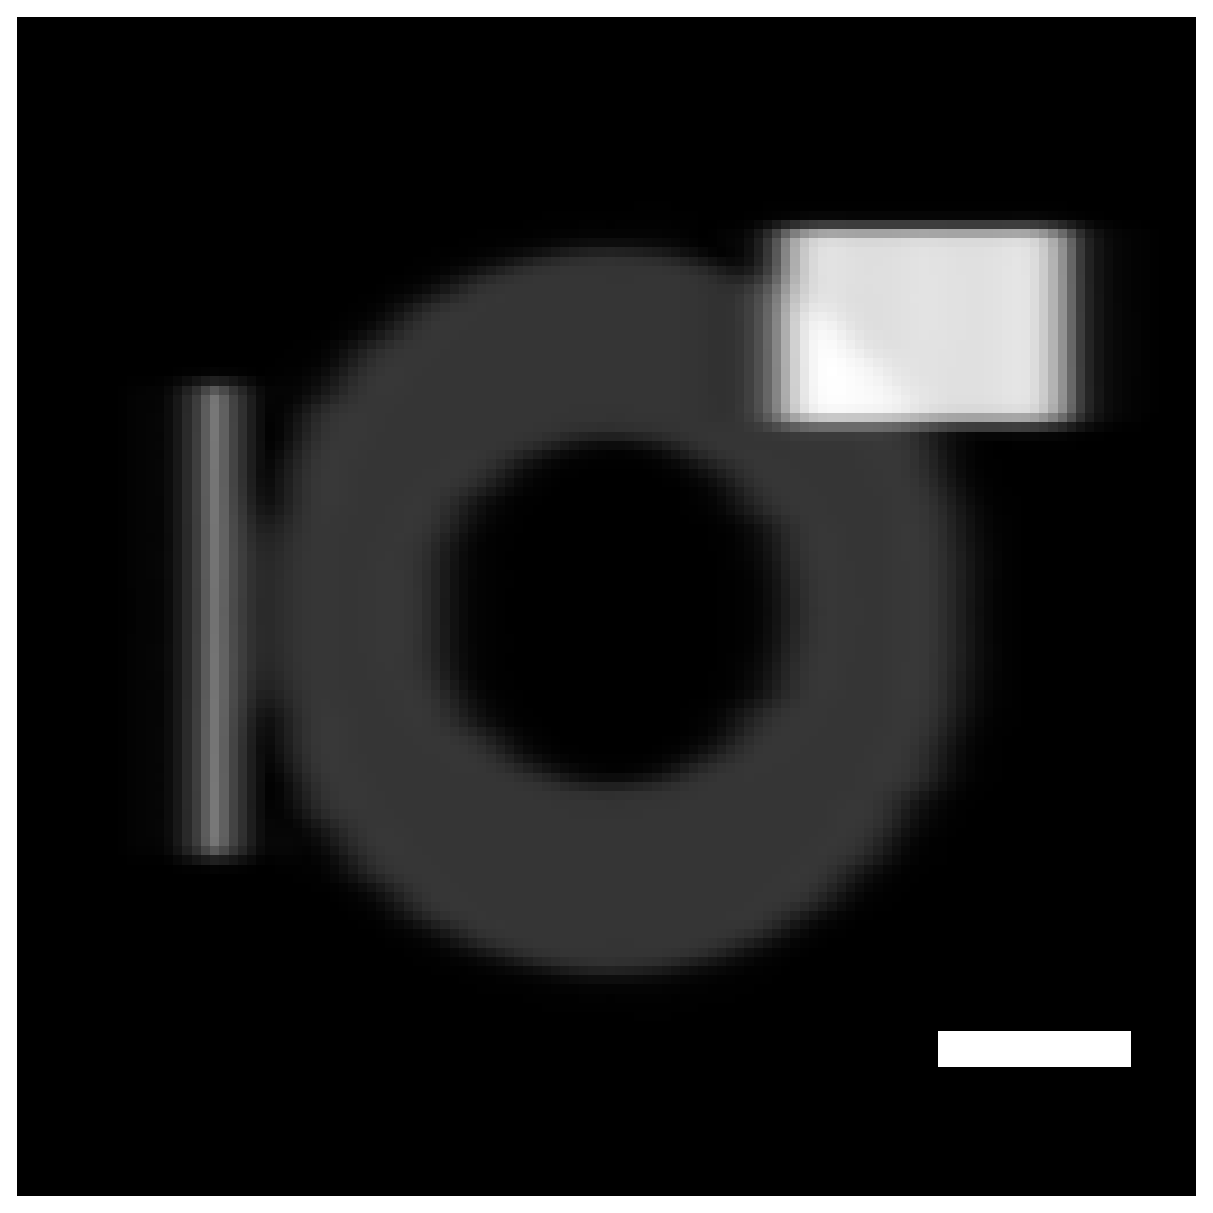
\includegraphics[width=4cm]{../app_hilo/isu2}}
  \subfigure[$I_\textrm{lp}$]{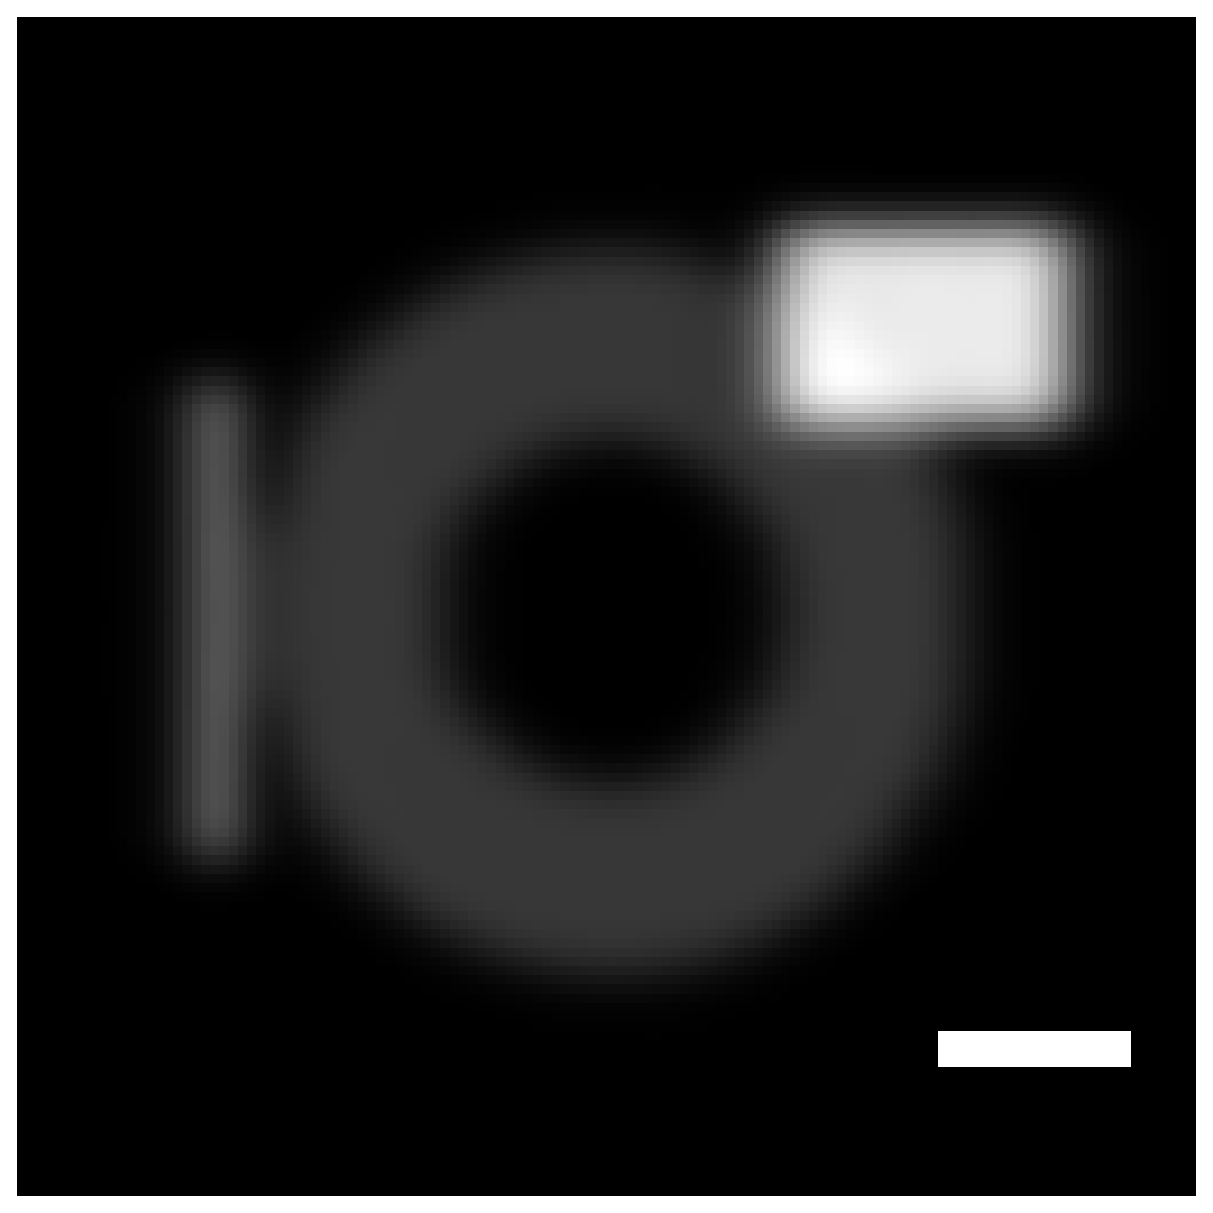
\includegraphics[width=4cm]{../app_hilo/ilp2}}
  \subfigure[$I_\textrm{hilo}$]{\label{fig:ihilo2}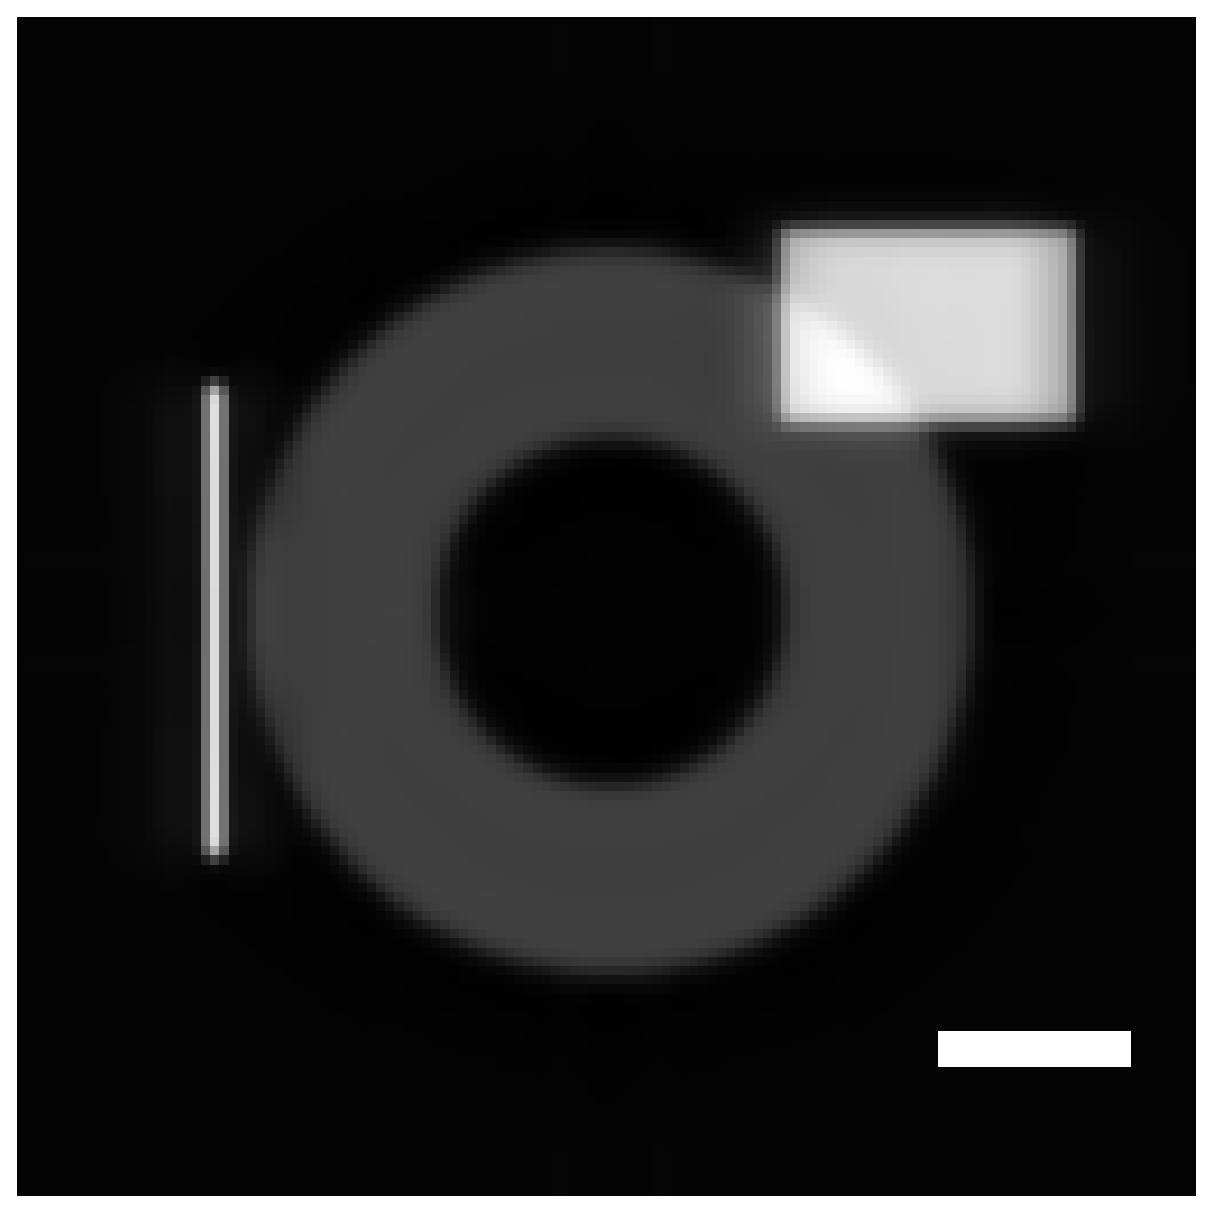
\includegraphics[width=4cm]{../app_hilo/ihilo2}}
  \caption{Intermediate results and the end result for the HiLo single
    side-band demodulation algorithm. The scalebars are
    \unit[2]{$\mu$m} wide.}
  \label{fig:hilo2_2}
\end{figure}
\subsubsection*{Discussion}
One advantage of the single side-band demodulation method compared to
the local variance estimation method is that it allows for a higher
cut-off frequency $k_c$ without introducing artifacts in the
intermediate image $I_{su}$. That accounts for the better appearance
of the result \figref{fig:ihilo2} compared to \figref{fig:ihilo} (at
least for this particular grating).

Probably the results would be even better, if a Sine pattern was
illuminated into the sample. Then, there would be no second orders in
\figref{fig:hilo2}~(b) and the filter would be easier to place.

Calculation of the ratio (single side-band demodulation) isn't the
only way to extract the modulated signal. Another approach involving
subtracting the widefield image\footnote{Suggested by R.~Heintzmann.}
and shifting in Fourier space is discussed in the following section.
\section{Alternative method (subtraction method)}
Instead of using a non-hermitian filter to extract the modulated part
of the non-uniformly illuminated image $I_n$ it is also possible to
employ the Fourier shift theorem: A shift in real space is 
a multiplication with a phase factor in k-space. 

Given two images in real space $f(\vect x)$ and $g(\vect x)$. The
image $g$ contains the same information as $f$ but shifted by a vector
$\vect a$. The theorem can be expressed like this:
\begin{align}
  g(\vect x)=f(\vect x+\vect a)
  \quad
  \rightarrow
  \quad
  \tilde g(\vect k)=e^{i\vect k\vect a}\tilde f(\vect k).
\end{align}
One can find the shift by searching for the maximum $\vect x_0=\vect a$ in
the cross-correlation $cov(\vect x)$:
\begin{align}
  cov(f,g)(\vect x)
  =\int f(\vect\chi) g(\vect x+\vect\chi) \textrm{d}\vect\chi
  =f(\vect x)\otimes g(-\vect x)
  =FT^{-1}(\tilde f(\vect k)\cdot\tilde g^*(\vect k)).
\end{align}
First the uniform image $I_u$ is subtracted from the image with the
grating $I_n$ in order to suppress the zero order. The following code
integrates over a circle around the origin in k-space to find a
constant {\sf kappa} to scale $I_u$ with. Furthermore the
Fourier transform of the images is divided by the OTF in order to
correct for the non-constant frequency transfer in the microscope
objective\footnote{Note that for this to work with noisy data a
  Wiener filter would be necessary.}
\begin{lstlisting}
kin=ft(in);
kiu=ft(iu);
% scale kin and kiu so that ic has no zero order
kappa=sum(abs(kin)./abs(kiu).*(rr(in)<5))./sum(rr(in)<5)
%% project otf along z
skpsf=squeeze(sum(kpsf,[],3));
corr=gaussf((rr(skpsf,'freq')<.42),3)./skpsf;
%% correct for the otf
ckin=corr.*kin;
ckiu=corr.*kiu;
%% correlate to find grating positions
ackin=abs(ckin-kappa.*ckiu);
ackiu=abs(ckiu).*(rr(ackiu,'freq')<.16 | abs(xx(ackiu,'freq'))<.06);
\end{lstlisting}
The Fourier transform of the OTF-corrected non-uniform image is shown
in \figref{fig:ackin}. It still contains the $\pm1$ orders. In order
to measure their exact position (depending on the grating period {\sf
  P}) the zero order of the widefield k-space is selected (in variable
{\sf ackiu}, \figref{fig:hilo3}~(b)) and cross-correlated with {\sf
  ackin} (\figref{fig:hilo3}~(a)).

\begin{figure}[htb]
  \centering \subfigure[{\sf
    ackin}]{\label{fig:ackin}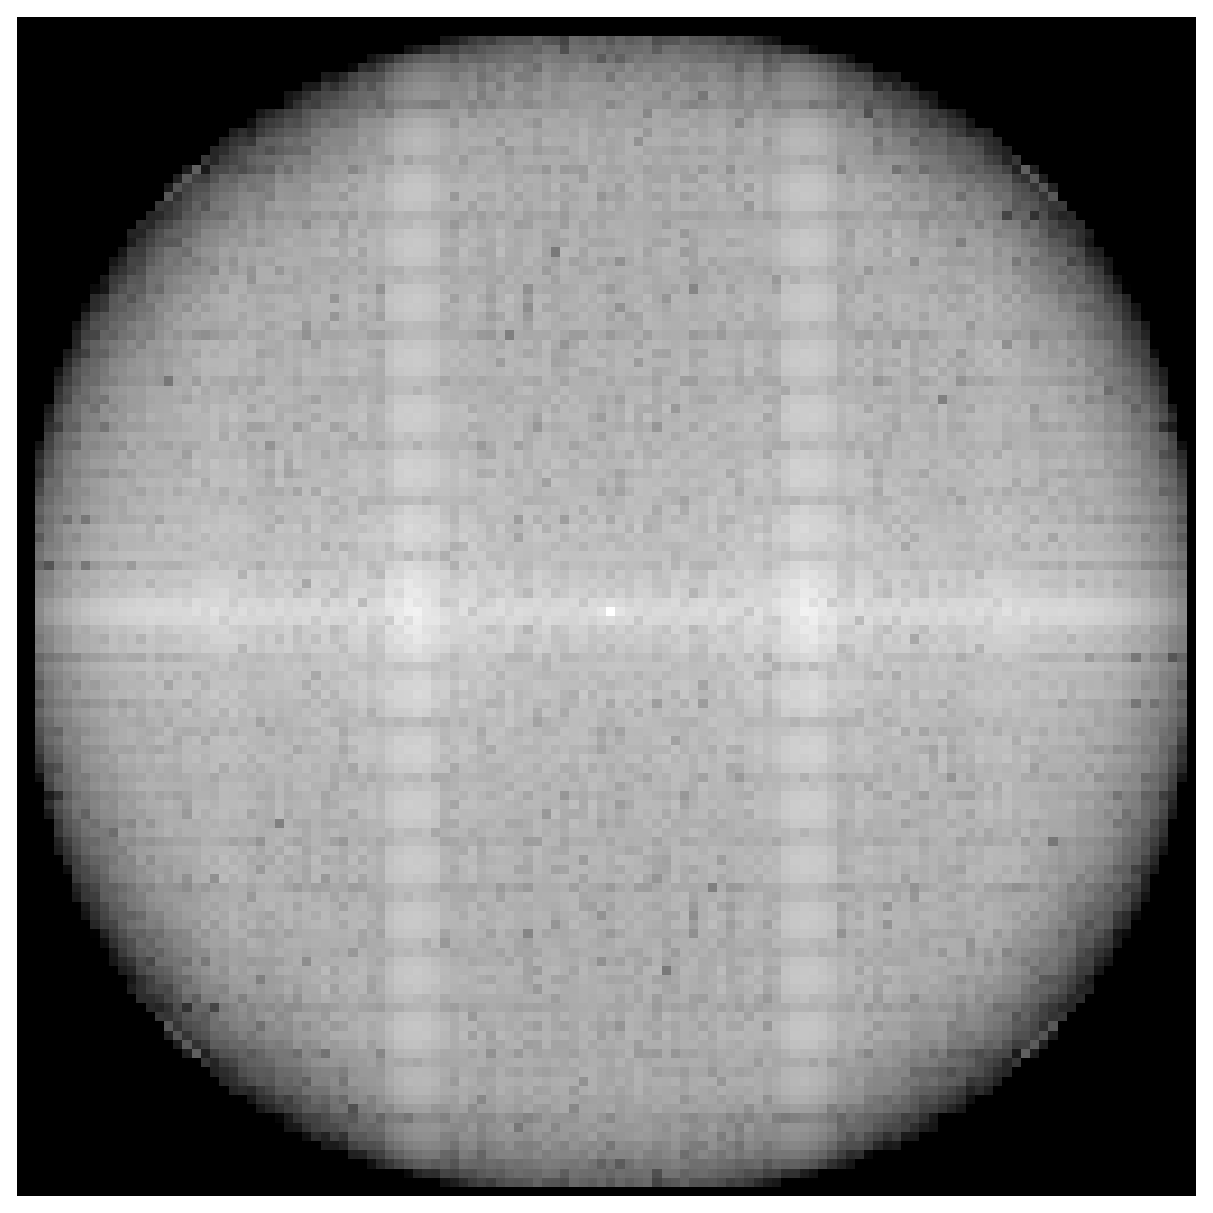
\includegraphics[width=6cm]{../app_hilo/ackin}}
  \subfigure[filtered zero order of uniform image $I_u$ {\sf
    ackiu}]{\label{fig:ackiu}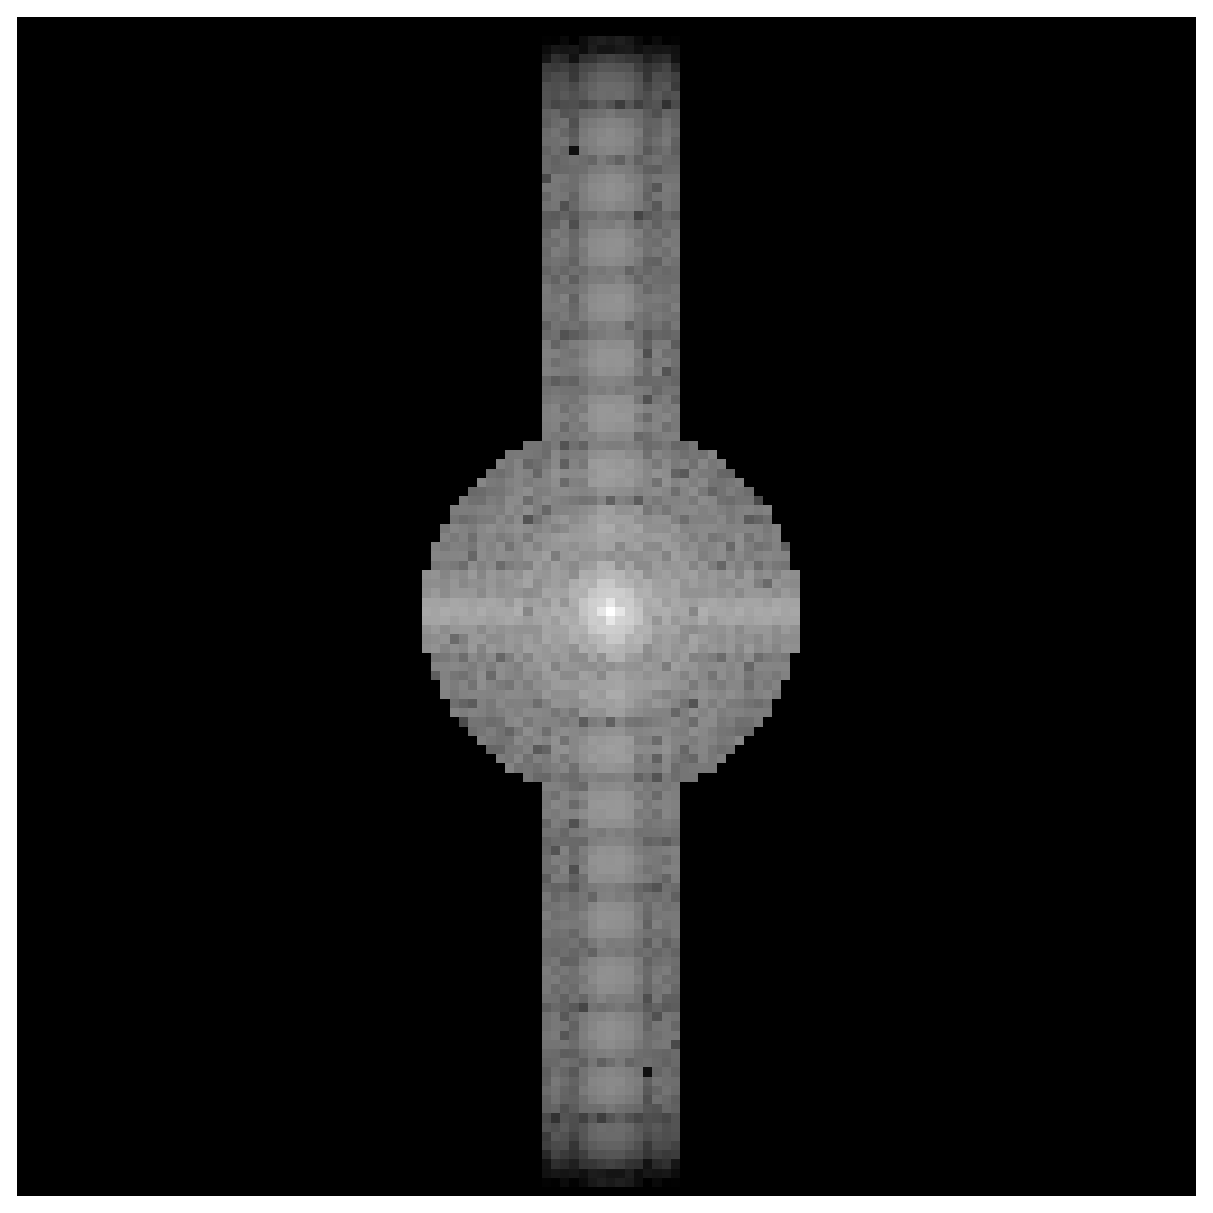
\includegraphics[width=6cm]{../app_hilo/ackiu}}
  \subfigure[Cross correlation
  $cov$.]{\label{fig:cov}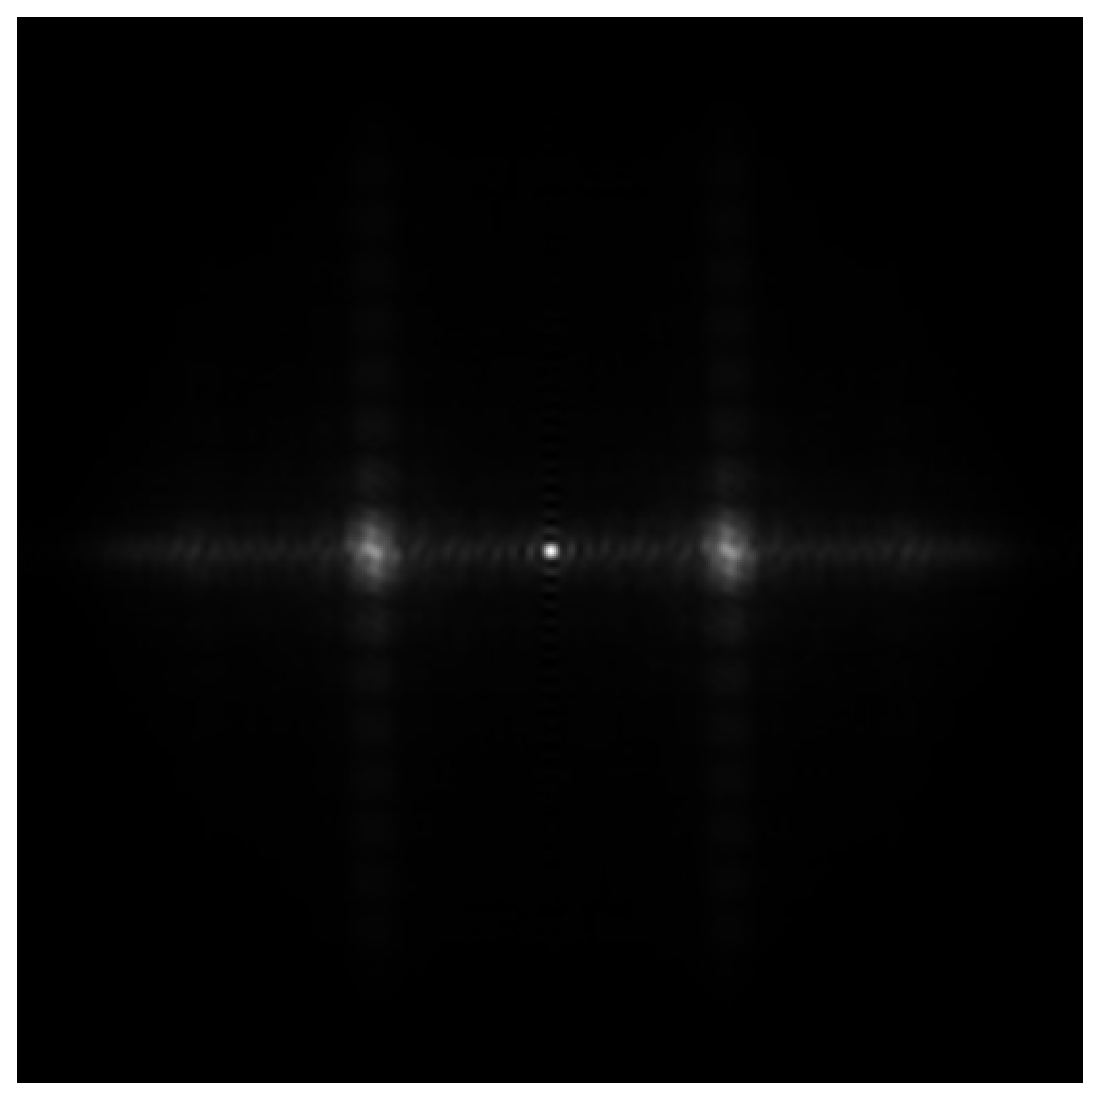
\includegraphics[width=6cm]{../app_hilo/cov}}
  \subfigure[Surface plot of
  $cov$.]{\label{fig:cov3d}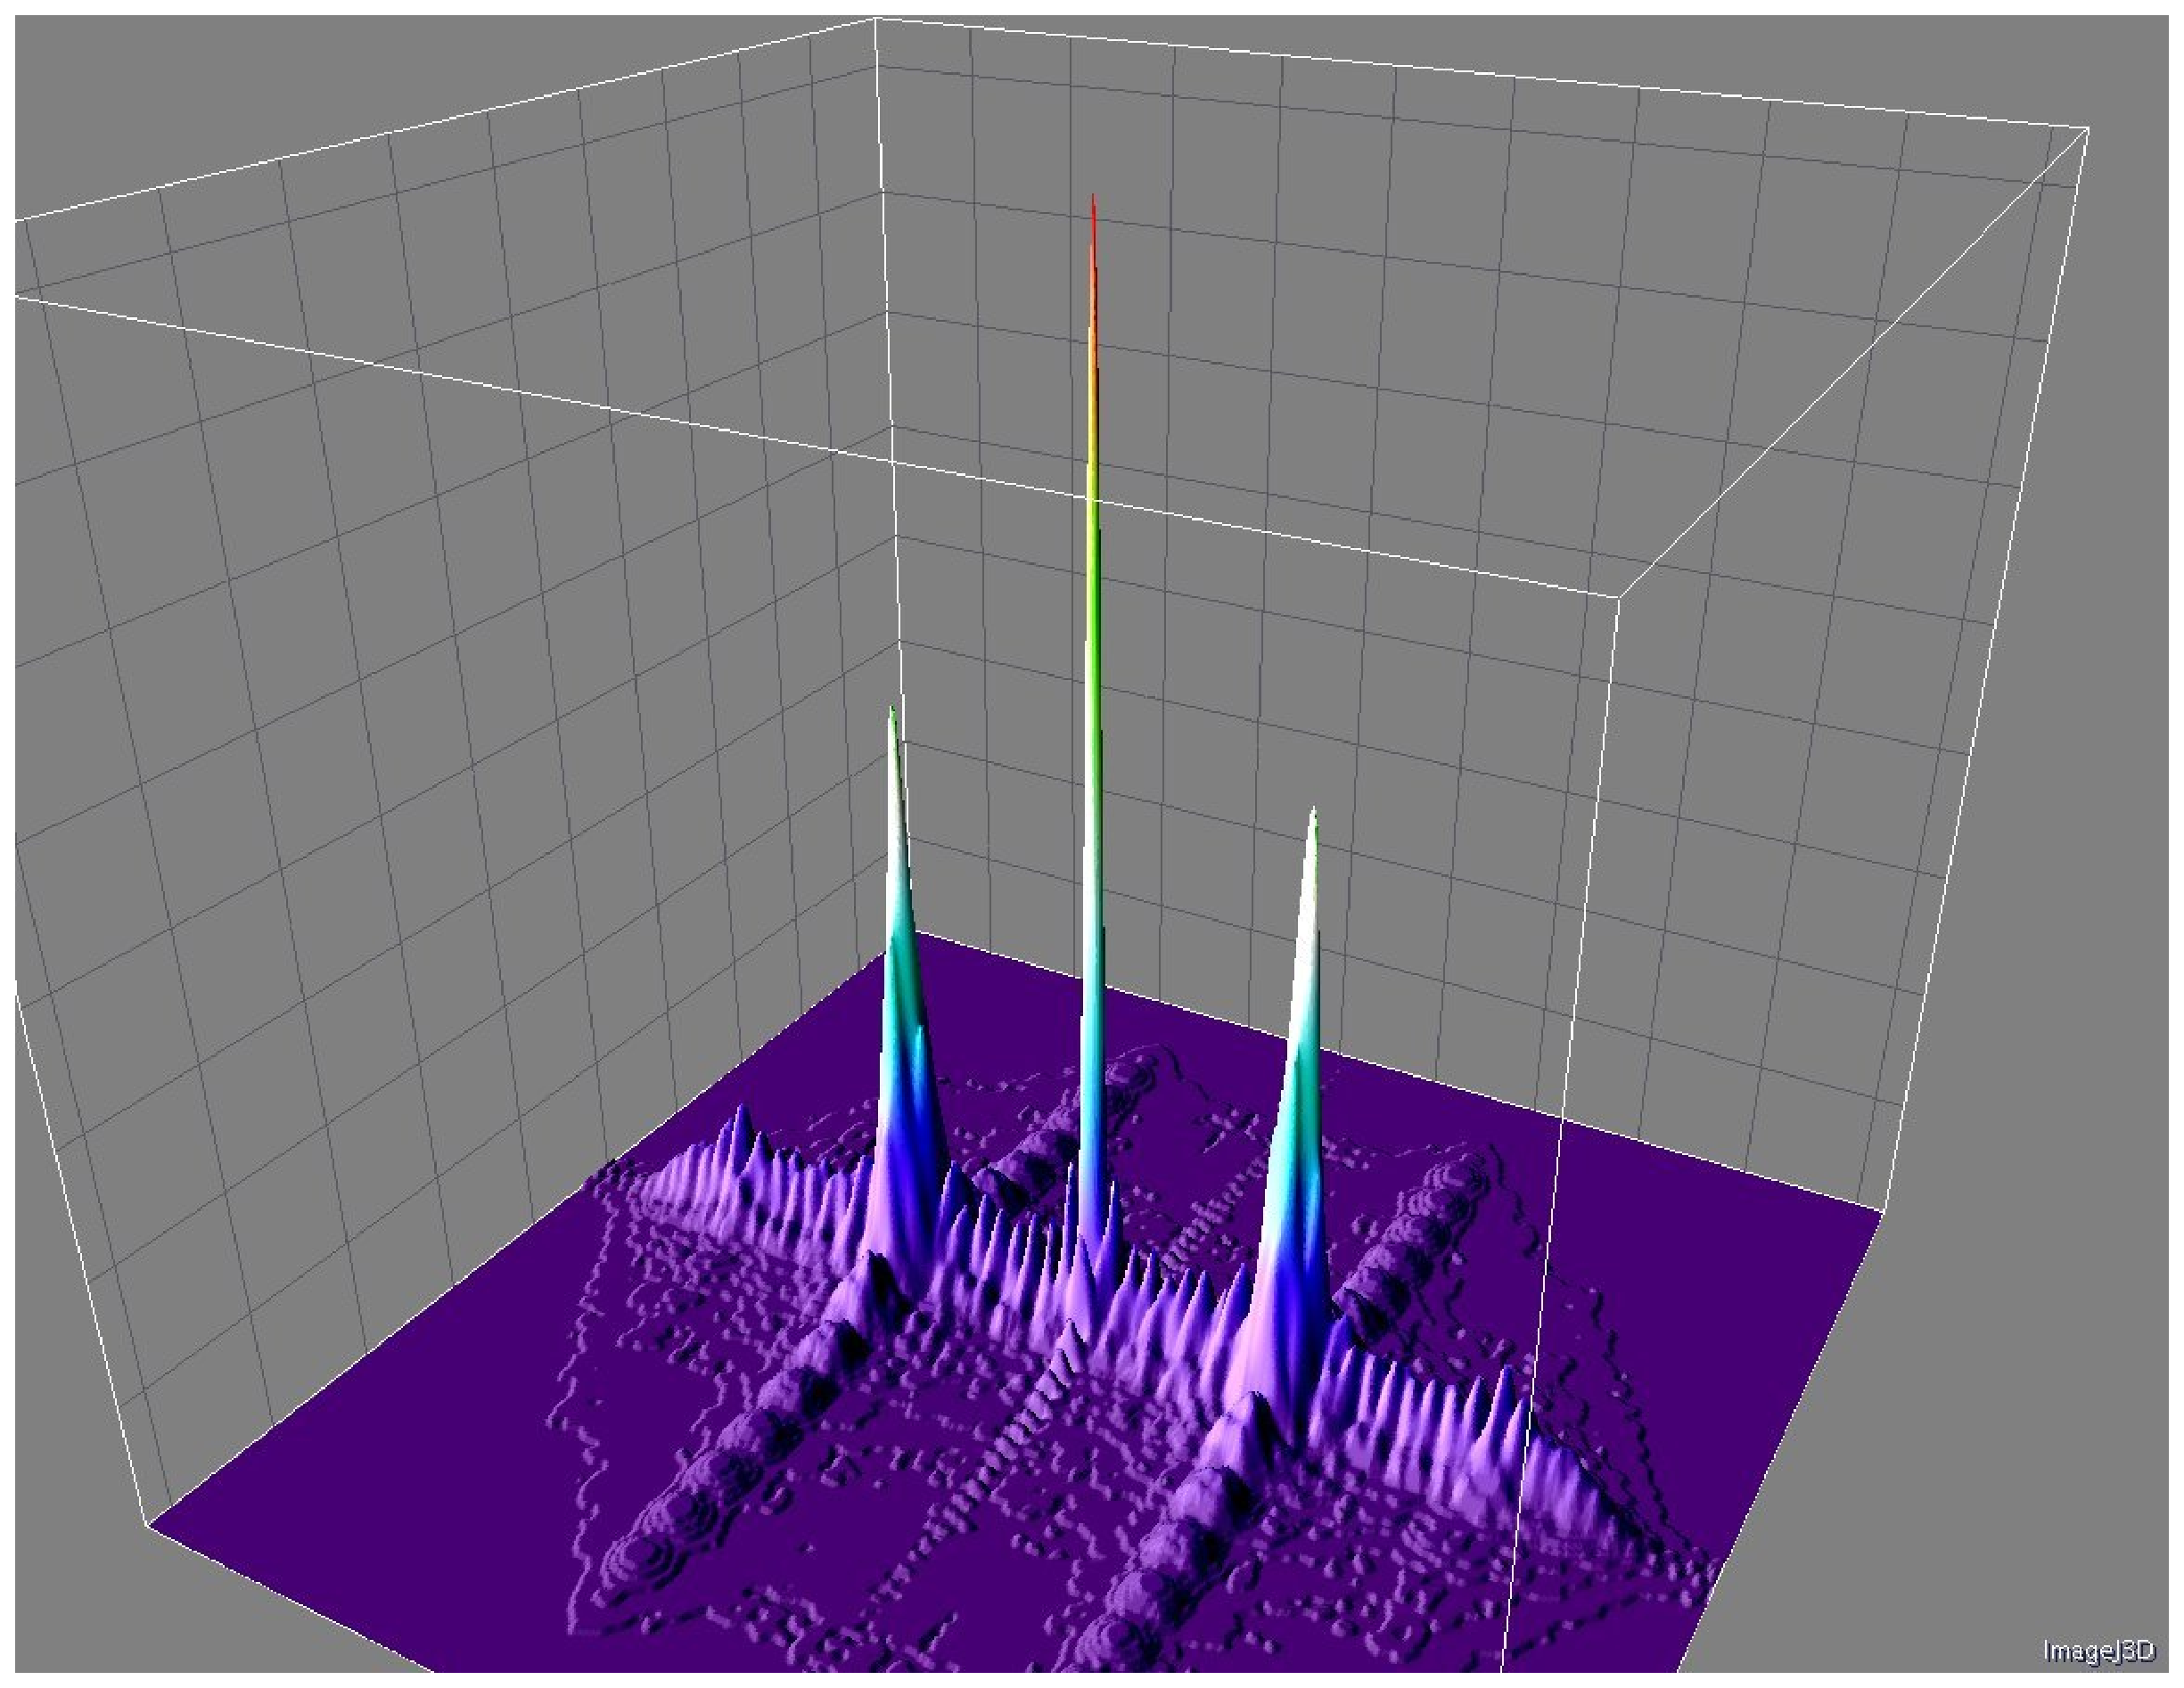
\includegraphics[width=6cm,viewport=100 0
    920 820,clip]{../app_hilo/cov3d}}
  \caption{Intermediate results for the HiLo ``shift'' algorithm.}
  \label{fig:hilo3}
\end{figure}
In order to locate the maximum in the cross-correlation with a
sufficient accuracy the convolution is done on a finer grid by
zero-padding the input images as shown in the following listing:
\begin{lstlisting}
kcov=ft(ackin).*conj(ft(ackiu));
% subsample the correlation by zero padding
kcov_big=newim(512,512)+i-i; % allocate complex array
st=256-64; w=127; en=st+w;
kcov_big(st:en,st:en)=kcov;
cov=abs(ift(kcov_big)); % this contains the cross correlation
\end{lstlisting}
The $512\times512$ image {\sf cov} is shown in \figref{fig:cov} and
\figref{fig:cov3d}. The next listing is the code to locate the centre
of gravity of the nine points on top of the right peak in
\figref{fig:hilo3}~(c,d):
\begin{lstlisting}
%% find maximum on the right of the correlation
startx=75*4;
[m,p]=max(abs(cov(startx:end,:)));
pos=[p(1)+startx,p(2)];
% determine center of mass of the 3x3 region around the maximum
region=abs(cov(pos(1)-1:pos(1)+1,pos(2)-1:pos(2)+1));
region=region-min(region);
cm=[sum(xx(region).*region),sum(yy(region).*region)];
shift=(pos+cm-[256,256])/4 % divide by 4 to undo subsampling
\end{lstlisting}
For the example the displacement {\sf shift} is $(21.25,0)$ relative
to the centre of the $128\times128$ image.
\begin{figure}[htb]
  \centering \subfigure[ $\tilde
  q_s$.]{\label{fig:kqs}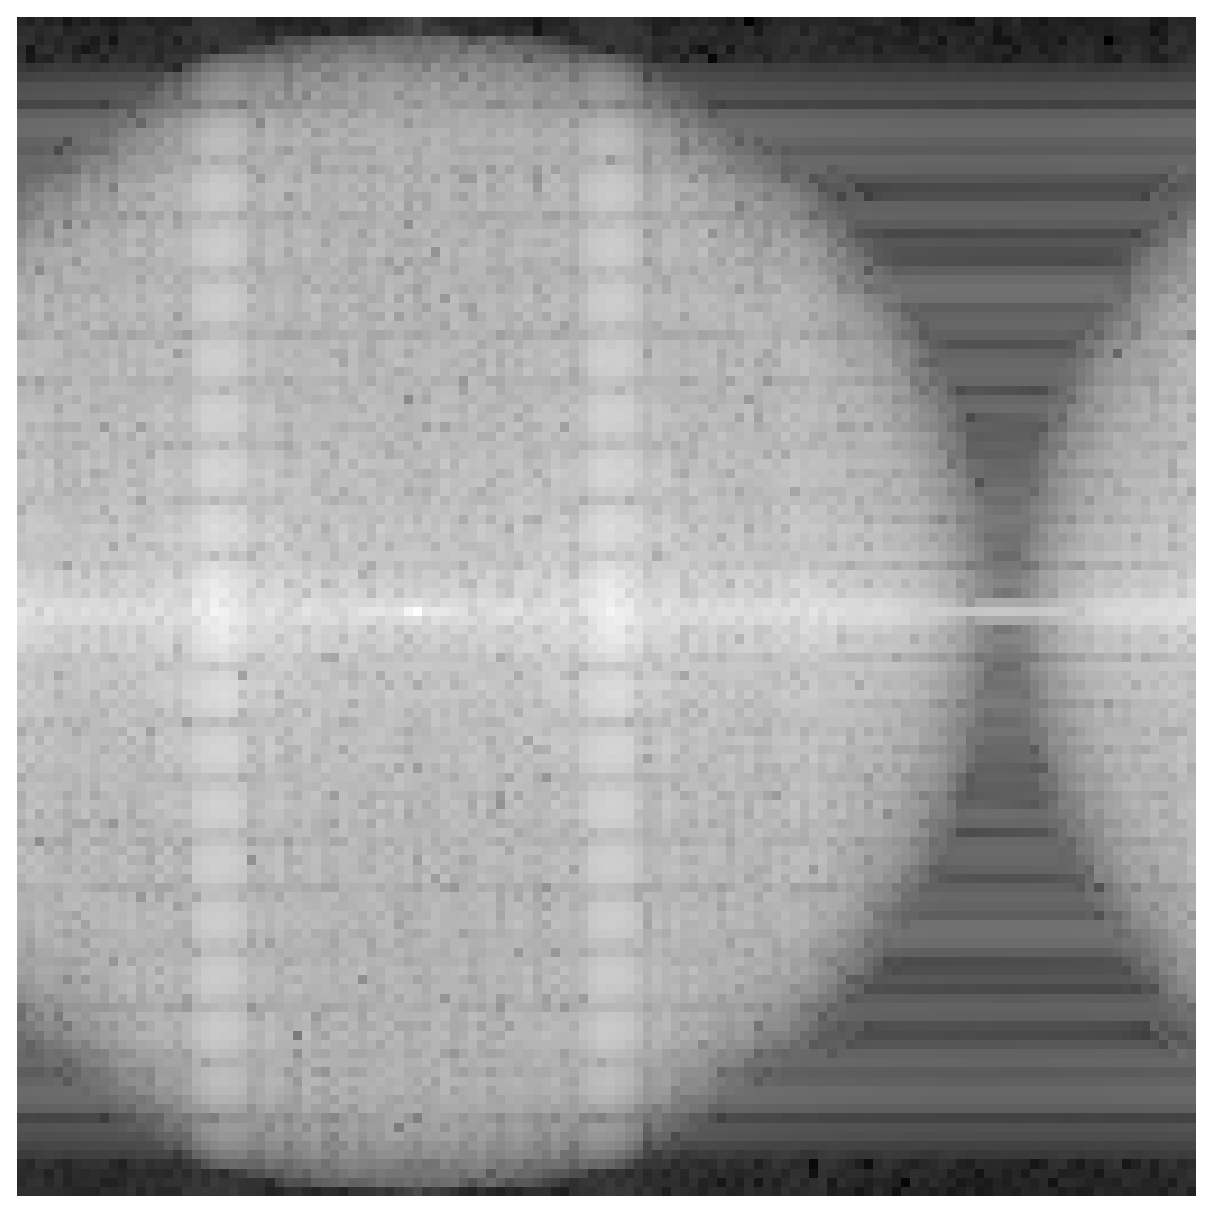
\includegraphics[width=4cm]{../app_hilo/kqs}}
  \subfigure[$\tilde q_s$ with low-pass
  applied.]{\label{fig:kqslp}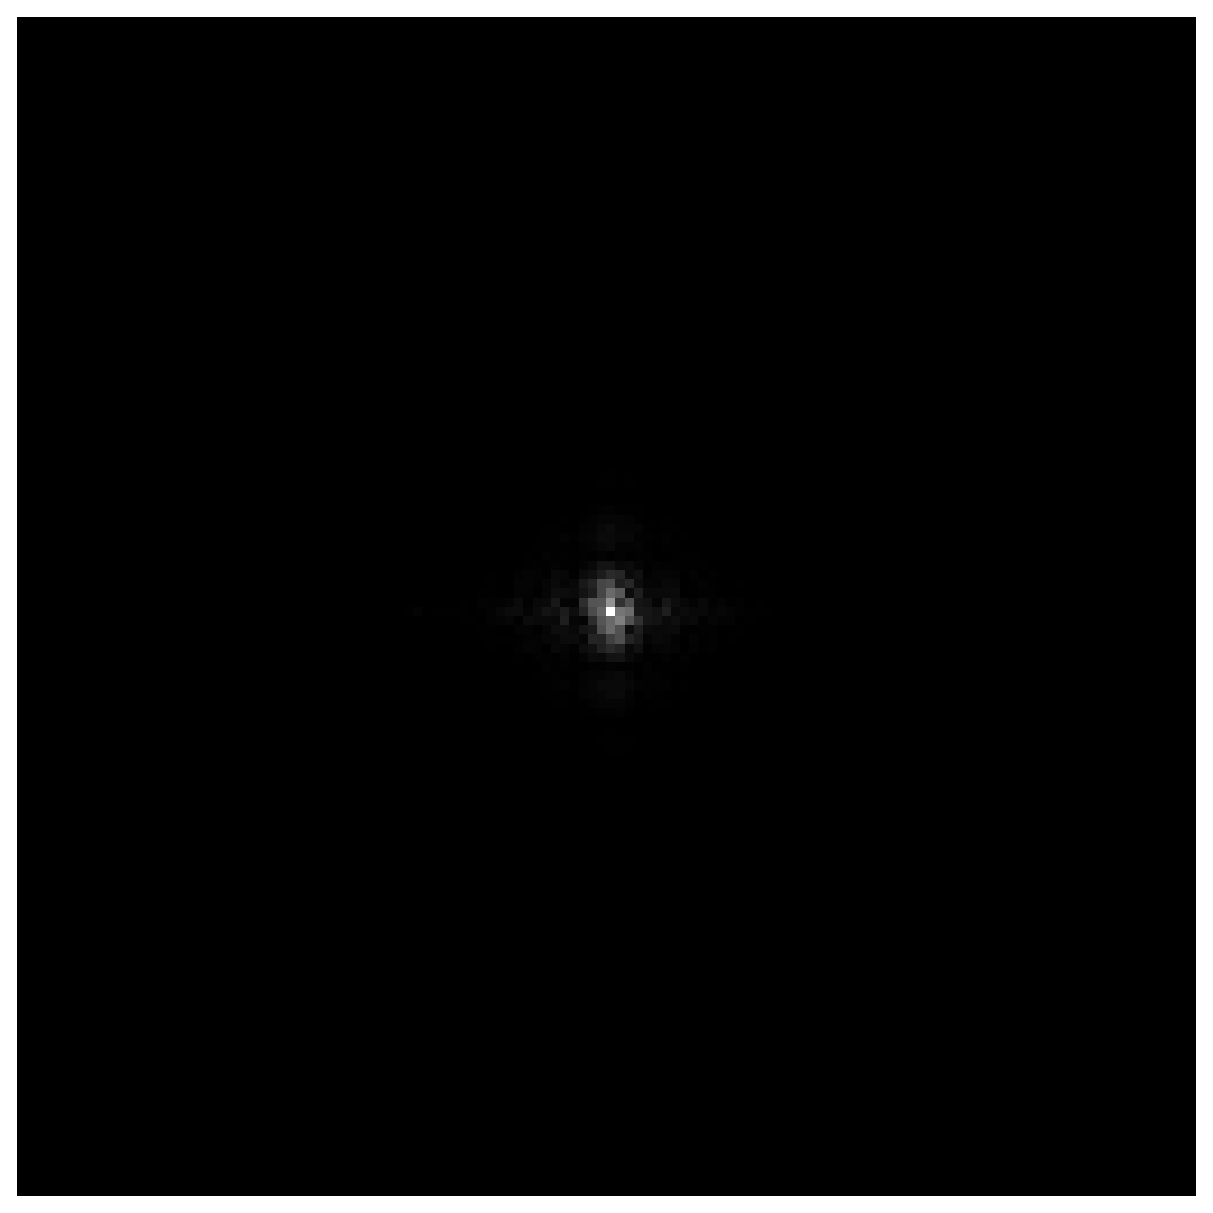
\includegraphics[width=4cm]{../app_hilo/kqslp}}
  \subfigure[$\tilde
  I_\textrm{hp}$]{\label{fig:kihp3}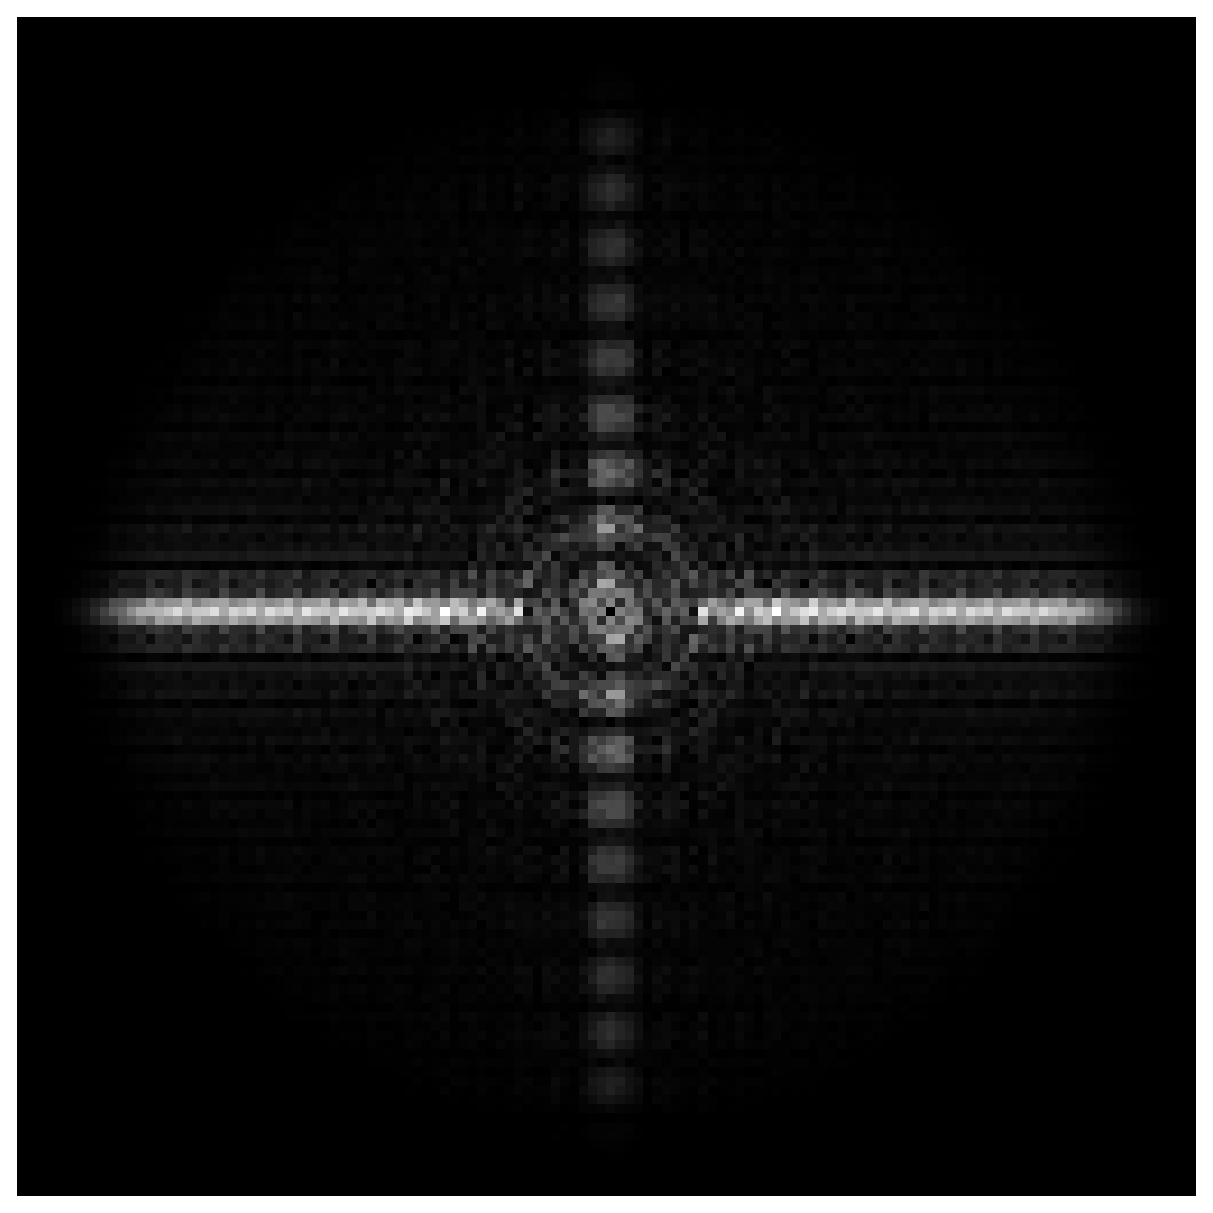
\includegraphics[width=4cm]{../app_hilo/kihp3}}
  \caption{The Fourier transform of the shifted zero-order-suppressed
    non-uniform image $q_s$ with (a) and without (b) low-pass filter
    and the Fourier transform of the corrected high-pass filtered
    uniform image (c). As opposed to all other k-space images (b) and
    (c) are not logarithmic.}
  \label{fig:hilo3_2}
\end{figure}
The following listing shows how the non-uniform image is shifted in
k-space so that the first order becomes DC. The result $\tilde q_s$
is shown in \figref{fig:kqs}.
\begin{lstlisting}
%% multiply by this in object space to shift +1 order into middle
doshift=exp(-i*2*pi*(xx(ckin,'freq').*shift(1)+...
        yy(ckin,'freq').*shift(2)));
kc=0.052;
r=rr(ckin,'freq');
klp=exp(-r.^2/(2*kc^2)); % low pass filter in k-space
q1=ift(ckin-kappa.*ckiu);
kqs=ft(q1.*doshift);
cm=abs(ift(kqs.*klp));
ihp=real(ift(ft(iu).*corr.*(1-klp)));
% integrate over ring with radius kc to find eta
ring=abs(ft(besselj(0,2*pi*kc*n.*r)));
ring2=r-1./n<kc & r+1./n>kc;
cring=ring.*ring2;
nring=cring./sum(abs(cring));
eta=sum(abs(ft(ihp))/abs(ft(cm)).*nring);
% combine highpass and lowpass filtered images
ihilo3=2.*cm+ihp; % don't use eta
\end{lstlisting}
The calculation of $\eta$ gives the value $1.16$. It turns out that
the reconstructed slice (\figref{fig:ihilo3}) looks better with a
value of $\eta=2$. This makes sense as the grating reduces the
illumination power approximately by this factor.
\begin{figure}[htb]
  \centering \subfigure[ {\sf
    cm}]{\label{fig:cm}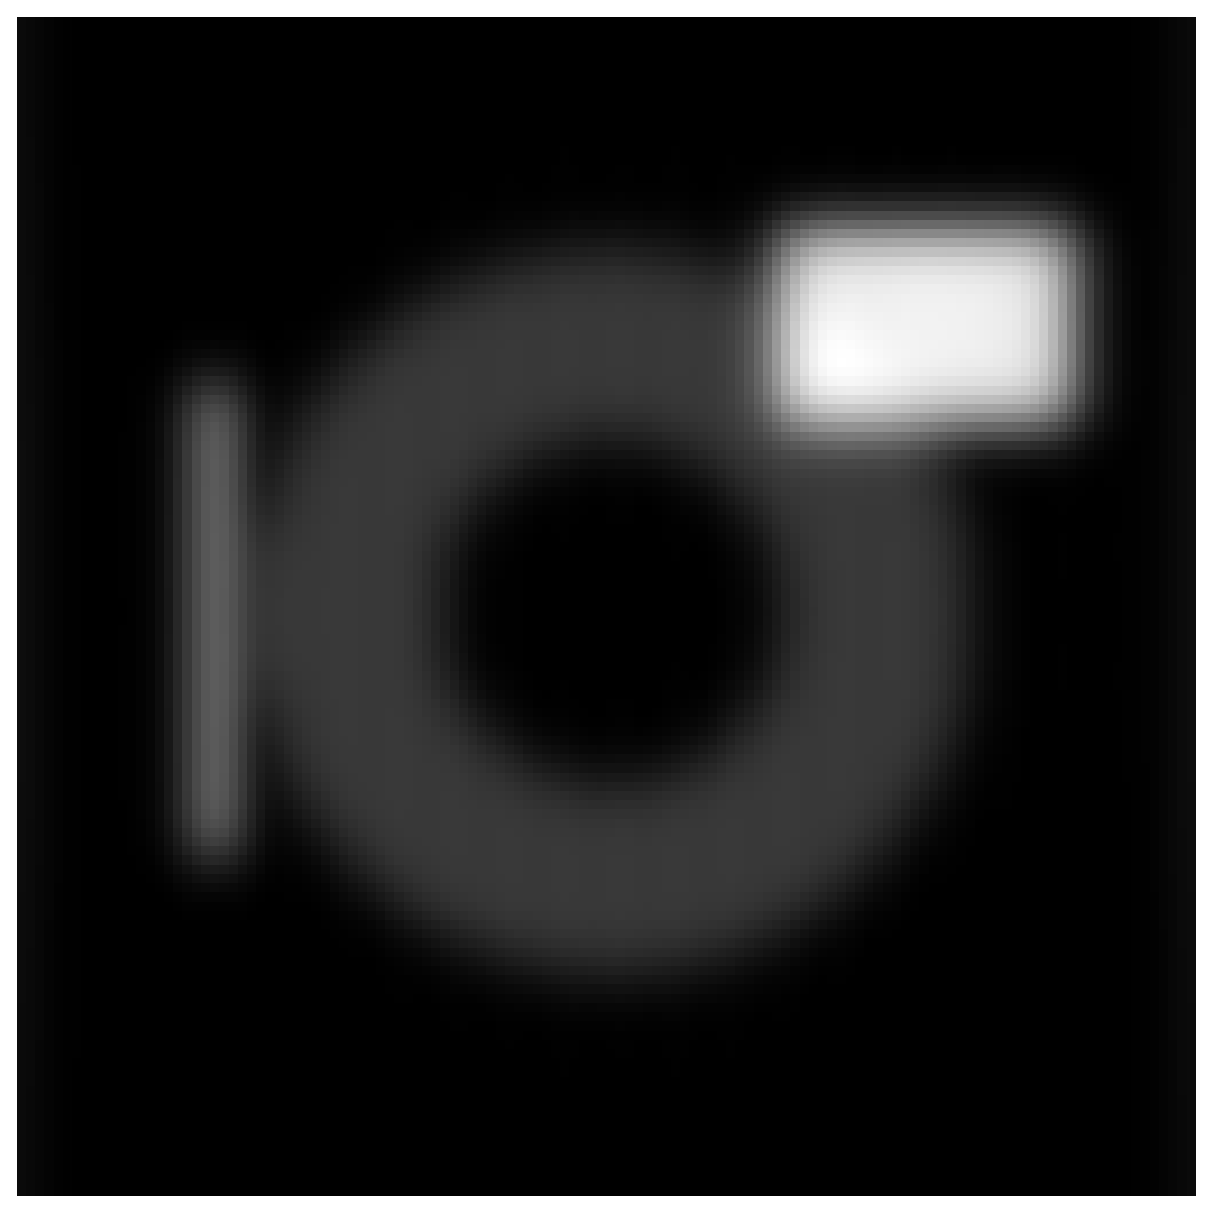
\includegraphics[width=4cm]{../app_hilo/cm}}
  \subfigure[$I_\textrm{hp}$]{\label{fig:ihp}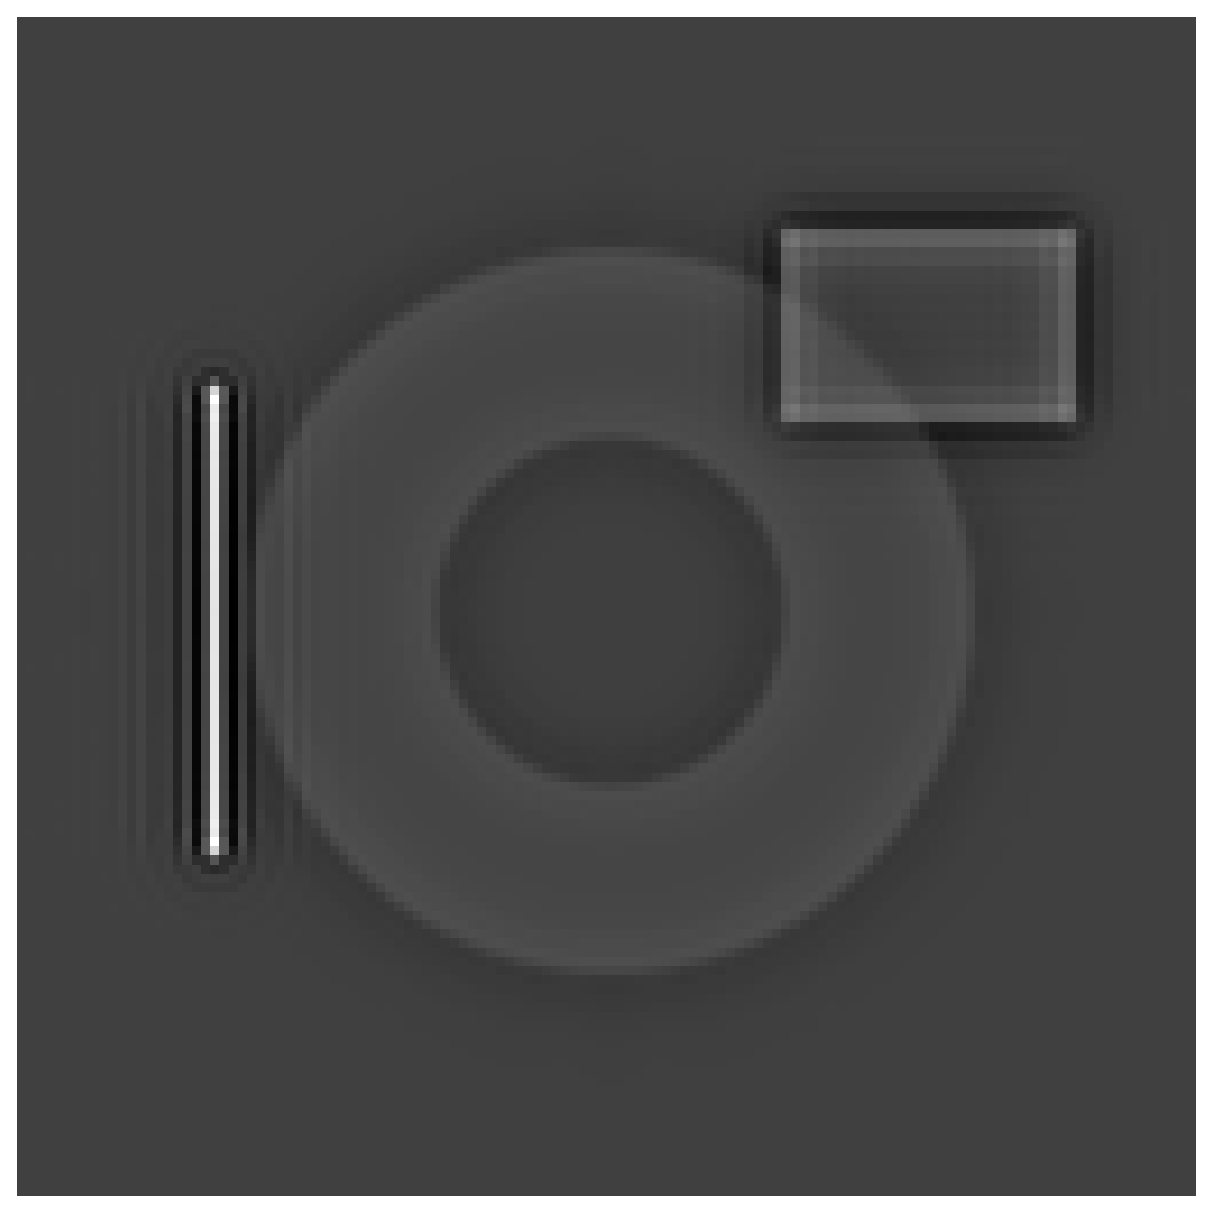
\includegraphics[width=4cm]{../app_hilo/ihp3}}
  \subfigure[$I_\textrm{hilo}$]{\label{fig:ihilo3}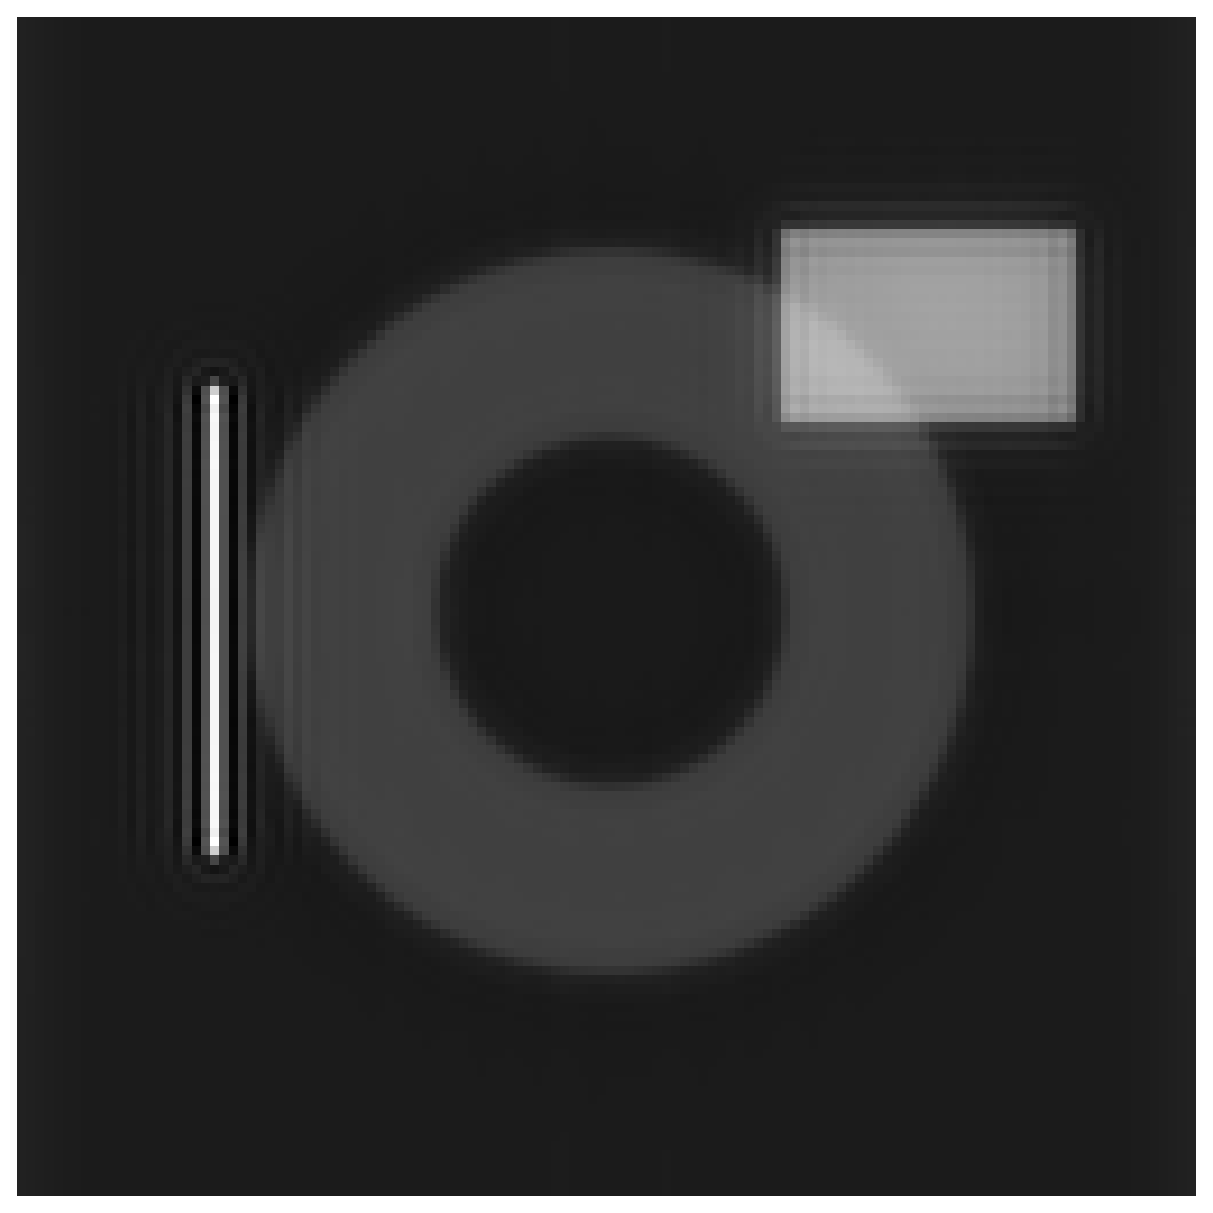
\includegraphics[width=4cm]{../app_hilo/ihilo3}}
  \caption{Low (a) and high-frequency (b) images in real space and the
    end result (c).}
  \label{fig:hilo3_3}
\end{figure}
\subsubsection{Discussion}
We believe conceptually the subtraction approach is simpler to
understand than the single side-band demodulation method. 

Indeed, long after this section was devised we found \cite{Mertz2010},
where they used a subtraction followed by a rectification
$\abs{I_u-2I_n}$ to partially demodulate the signal.

As a follow up it might be instructive to investigate the performance
of the three different demodulation approaches in the presence of
noise.
